\section*{Database Project Report Template}

\textbf{Project ID \& Title:} \#2: On-Demand Streaming Platform (Mini-Netflix)

\subsection*{A. Project Identity}

\begin{itemize}
\item
  \textbf{Team Name:} No Man's Land (NML)
\end{itemize}

\begin{itemize}
\item
  \textbf{Team Members:} Trần Duy Nhân (\nolinkurl{n25dece106@student.ptithcm.edu.vn}), Võ Lâm (\nolinkurl{n25dece055@student.ptithcm.edu.vn}), Tô Minh Hưng (\nolinkurl{n25dece092@student.ptithcm.edu.vn})
\end{itemize}

\begin{itemize}
\item
  \textbf{Project Title:} Mini-Netflix On-Demand Streaming Platform: Managing Complex Content Hierarchies and Tiered Membership Access through EER Modeling and Relational Normalization
\end{itemize}

\subsection*{B. Report structure}

\section*{1. Introduction \& Project Scope (Adapted from ISO/IEC/IEEE 29148)}

\subsection*{1.1 Business \& Product Overview}

\subsubsection*{1.1.1. Product Definition}

The proposed system is an On-Demand Streaming Platform (Mini-Netflix). The platform is a centralized multimedia delivery service designed to manage, categorize and stream digital video content to end-users.

To accurately manage this catalog, the system categorizes "Content" into two distinct hierarchical types:

Movies: Standalone video files characterized by a single duration and video resolution.

TV Series Episodes: Serialized media units that belong to a broader TV Series container, requiring complex tracking of seasons and episode numbers.

\subsubsection*{1.1.2. Customer \& User Definition}

The platform differentiates between administrative staff and end-user viewing through a strict hierarchical structure:

Database Administrator (DBA): The chief administrator who oversees and manages the database and DBMS resources. The DBA is strictly a backend role responsible for authorizing access, monitoring database use, coordinating hardware/software acquisition, and securing overall system performance.

Account Owner (The Customer): The master billing account responsible for administrative duties and purchasing the service. This entity acts as the primary \textquotesingle Customer\textquotesingle{} who manages the subscription tier (Free, Basic, Standard, or Premium), handles billing status, and has the authority to create or delete sub-profiles.

Profile (The Viewer): The actual end-user entity partitioned under a parent Account. Viewing sessions cannot happen at the Account level; they must be done through a Profile. Profiles are restricted to viewing content and managing personal preferences (e.g., language, avatars). Profiles can be designated as a "Kids Profile," which restricts their access to specific age-appropriate rating classifications.

\subsubsection*{1.1.3. Value Proposition}

The core business objective is to deliver a seamless and engaging user experience through three primary value pillars:

Personalized Viewing Experiences: By isolating viewing metrics into distinct M:N associative entities (Watchlist, Watch History, and Profile Ratings), the platform ensures that mutations or actions on Profile A never affect the recommendations or history of Profile B.

Tiered Access Control: The platform incentivizes upgrades by enforcing role-based content access. A user\textquotesingle s subscription tier dictates their maximum video quality, the number of allowed concurrent streams, and access to premium catalog items.

Structured Content Discovery: Utilizing a classification lookup catalog for genres and strict metadata tracking (release years, ratings), the platform allows users to efficiently navigate large libraries of both standalone movies and serialized TV shows.

\subsection*{1.2. System Objective}

\subsubsection*{1.2.1. Scenario Overview \& Technical Environment}

The proposed database system models the core backend architecture of an On-Demand Streaming Platform (Mini-Netflix). In this Universe of Discourse (UoD), the system orchestrates subscriber billing, multi-user profile separation, tiered content catalogs, active streaming sessions, and personalized watch metrics.

\subsubsection*{1.1.2 Core Purpose \& System Objectives}

The primary objective is to implement a robust, scalable, and normalized relational database schema (up to BCNF) that achieves:

• EER Content Specialization: Structuring a Content superclass with specialized Movie and TV Episode subclasses, avoiding null-heavy schemas.

• Subscription Tier Access Control: Enforcing role-based content access and concurrent stream limits directly via relational constraints.

• Partitioned Profile Telemetry: Isolating viewing histories, ratings, and watchlists per profile using resolved M:N associative entities.

• Strict Referential Integrity:000 Enforcing composite keys, foreign keys, and ON DELETE CASCADE policies to eliminate orphaned records.

\subsection*{1.3 Business Rules \& Constraints .}

\subsubsection*{1.3.1 Operational Constraints \& Semantic Integrity}

\subsubsection*{1.3.1.1 Tier \& Concurrency Rules}

• BR-01 (Access Authorization): A Profile can only access Content where Content.required\_\allowbreak{}tier\_\allowbreak{}id \textless= Account.tier\_\allowbreak{}id.

• BR-02 (Stream Caps): Active concurrent records in Active\_\allowbreak{}Session for a given account\_\allowbreak{}id ca  nnot exceed Subscription\_\allowbreak{}Tier.max\_\allowbreak{}concurrent\_\allowbreak{}streams.

\subsubsection*{1.3.1.2 Profile Isolation \& Parental Control}

• BR-03 (Data Isolation): Watch\_\allowbreak{}History, ratings, and Watchlist rows are strictly scoped to profile\_\allowbreak{}id. Mutations on Profile A must never affect Profile B.

• BR-04 (Kids Filter): If Profile.is\_\allowbreak{}kids\_\allowbreak{}profile = TRUE, queries must exclude Content with rating\_\allowbreak{}classification IN (\textquotesingle R\textquotesingle, \textquotesingle TV-MA\textquotesingle).

\subsubsection*{1.3.1.3 Cardinality \& Referential Bounds}

• BR-05 (Profile Threshold): Count of Profiles per account\_\allowbreak{}id must satisfy 1 \textless= Count \textless= 5.

• BR-06 (Cascade Protocol): ON DELETE CASCADE applies from Account -\textgreater{} Profile -\textgreater{} (Watchlist, Watch\_\allowbreak{}History, Active\_\allowbreak{}Session).

\subsubsection*{1.3.1.4 User Interaction \& Service Access}

BR-07 (Service Prerequisite): An unregistered user cannot interact with the streaming catalog. The creation of a valid Account is required to interact with the database.

BR-08 (Profile Enforcement): An Account cannot directly initiate a streaming session or save content. All viewing telemetry (Active\_\allowbreak{}Session), Watch\_\allowbreak{}History, and Watchlist records must be strictly tied to a Profile entity.

BR-09 (Demo/Free Tier Limitation): If an Account is registered but has an inactive billing\_\allowbreak{}status or belongs to a "Free/Guest" tier, its associated Profiles are restricted to accessing Content categorized exclusively as \textquotesingle Demo\textquotesingle{} or \textquotesingle Trailer\textquotesingle.

\subsubsection*{1.3.1.5 Billing \& Subscription Lifecycle Constraints}

BR-10 (Default Free-Tier Onboarding): Every newly registered Account must initialize with current\_\allowbreak{}tier\_\allowbreak{}id = 0 (Free tier) and an \textquotesingle Active\textquotesingle{} billing status. Paid subscription tiers (Basic, Standard, Premium) cannot be assigned at initial account creation without completing payment method onboarding.

BR-11 (Payment Method Prerequisite for Paid Tiers): An Account must have at least one valid tokenized payment method recorded in Credit\_\allowbreak{}Card (COUNT(*) \textgreater= 1 for that account\_\allowbreak{}id) before upgrading current\_\allowbreak{}tier\_\allowbreak{}id to any paid tier (tier\_\allowbreak{}id \textgreater{} 0) or processing a paid subscription renewal. Attempts to upgrade or renew without a registered payment card are rejected (HTTP 402 Payment Required).

BR-12 (Recurring Billing Cycle): The system mandates a recurring 30-day billing cycle starting from the Account.registration\_\allowbreak{}date. The billed amount must strictly map to the monthly\_\allowbreak{}price of the Account\textquotesingle s currently assigned Subscription\_\allowbreak{}Tier

BR-13 (Delinquency \& Suspension): If an Account fails to process a payment, its billing\_\allowbreak{}status updates to \textquotesingle Overdue\textquotesingle{} or \textquotesingle Suspended\textquotesingle. When this occurs, the system must immediately revoke premium access for all associated Profiles, dropping their viewing privileges down to the "Demo/Free" constraints (as defined in BR-09).

BR-14 (Tier Modifications): Provided the account satisfies BR-11 (at least one registered Credit\_\allowbreak{}Card on file), if an Account Owner chooses to upgrade their Subscription\_\allowbreak{}Tier (e.g., Free to Basic or Premium), the change and new access limits take effect immediately. If the user downgrades, the change takes effect at the beginning of the next billing cycle.

BR-15 (Cancellation \& Data Retention): Canceling a subscription sets the billing\_\allowbreak{}status to \textquotesingle Inactive\textquotesingle. The system does not immediately execute the ON DELETE CASCADE protocol. Instead, Profiles, Watchlist, and Watch\_\allowbreak{}History records are retained for a 10-month grace period to allow the user to reactivate their account without losing their personalized data.

\section*{2. Database Design (ISO/IEC 19505 / IE Standards)}

\noindent\begin{minipage}{\linewidth}
\subsection*{2.1 Conceptual Model (EER Diagram)}
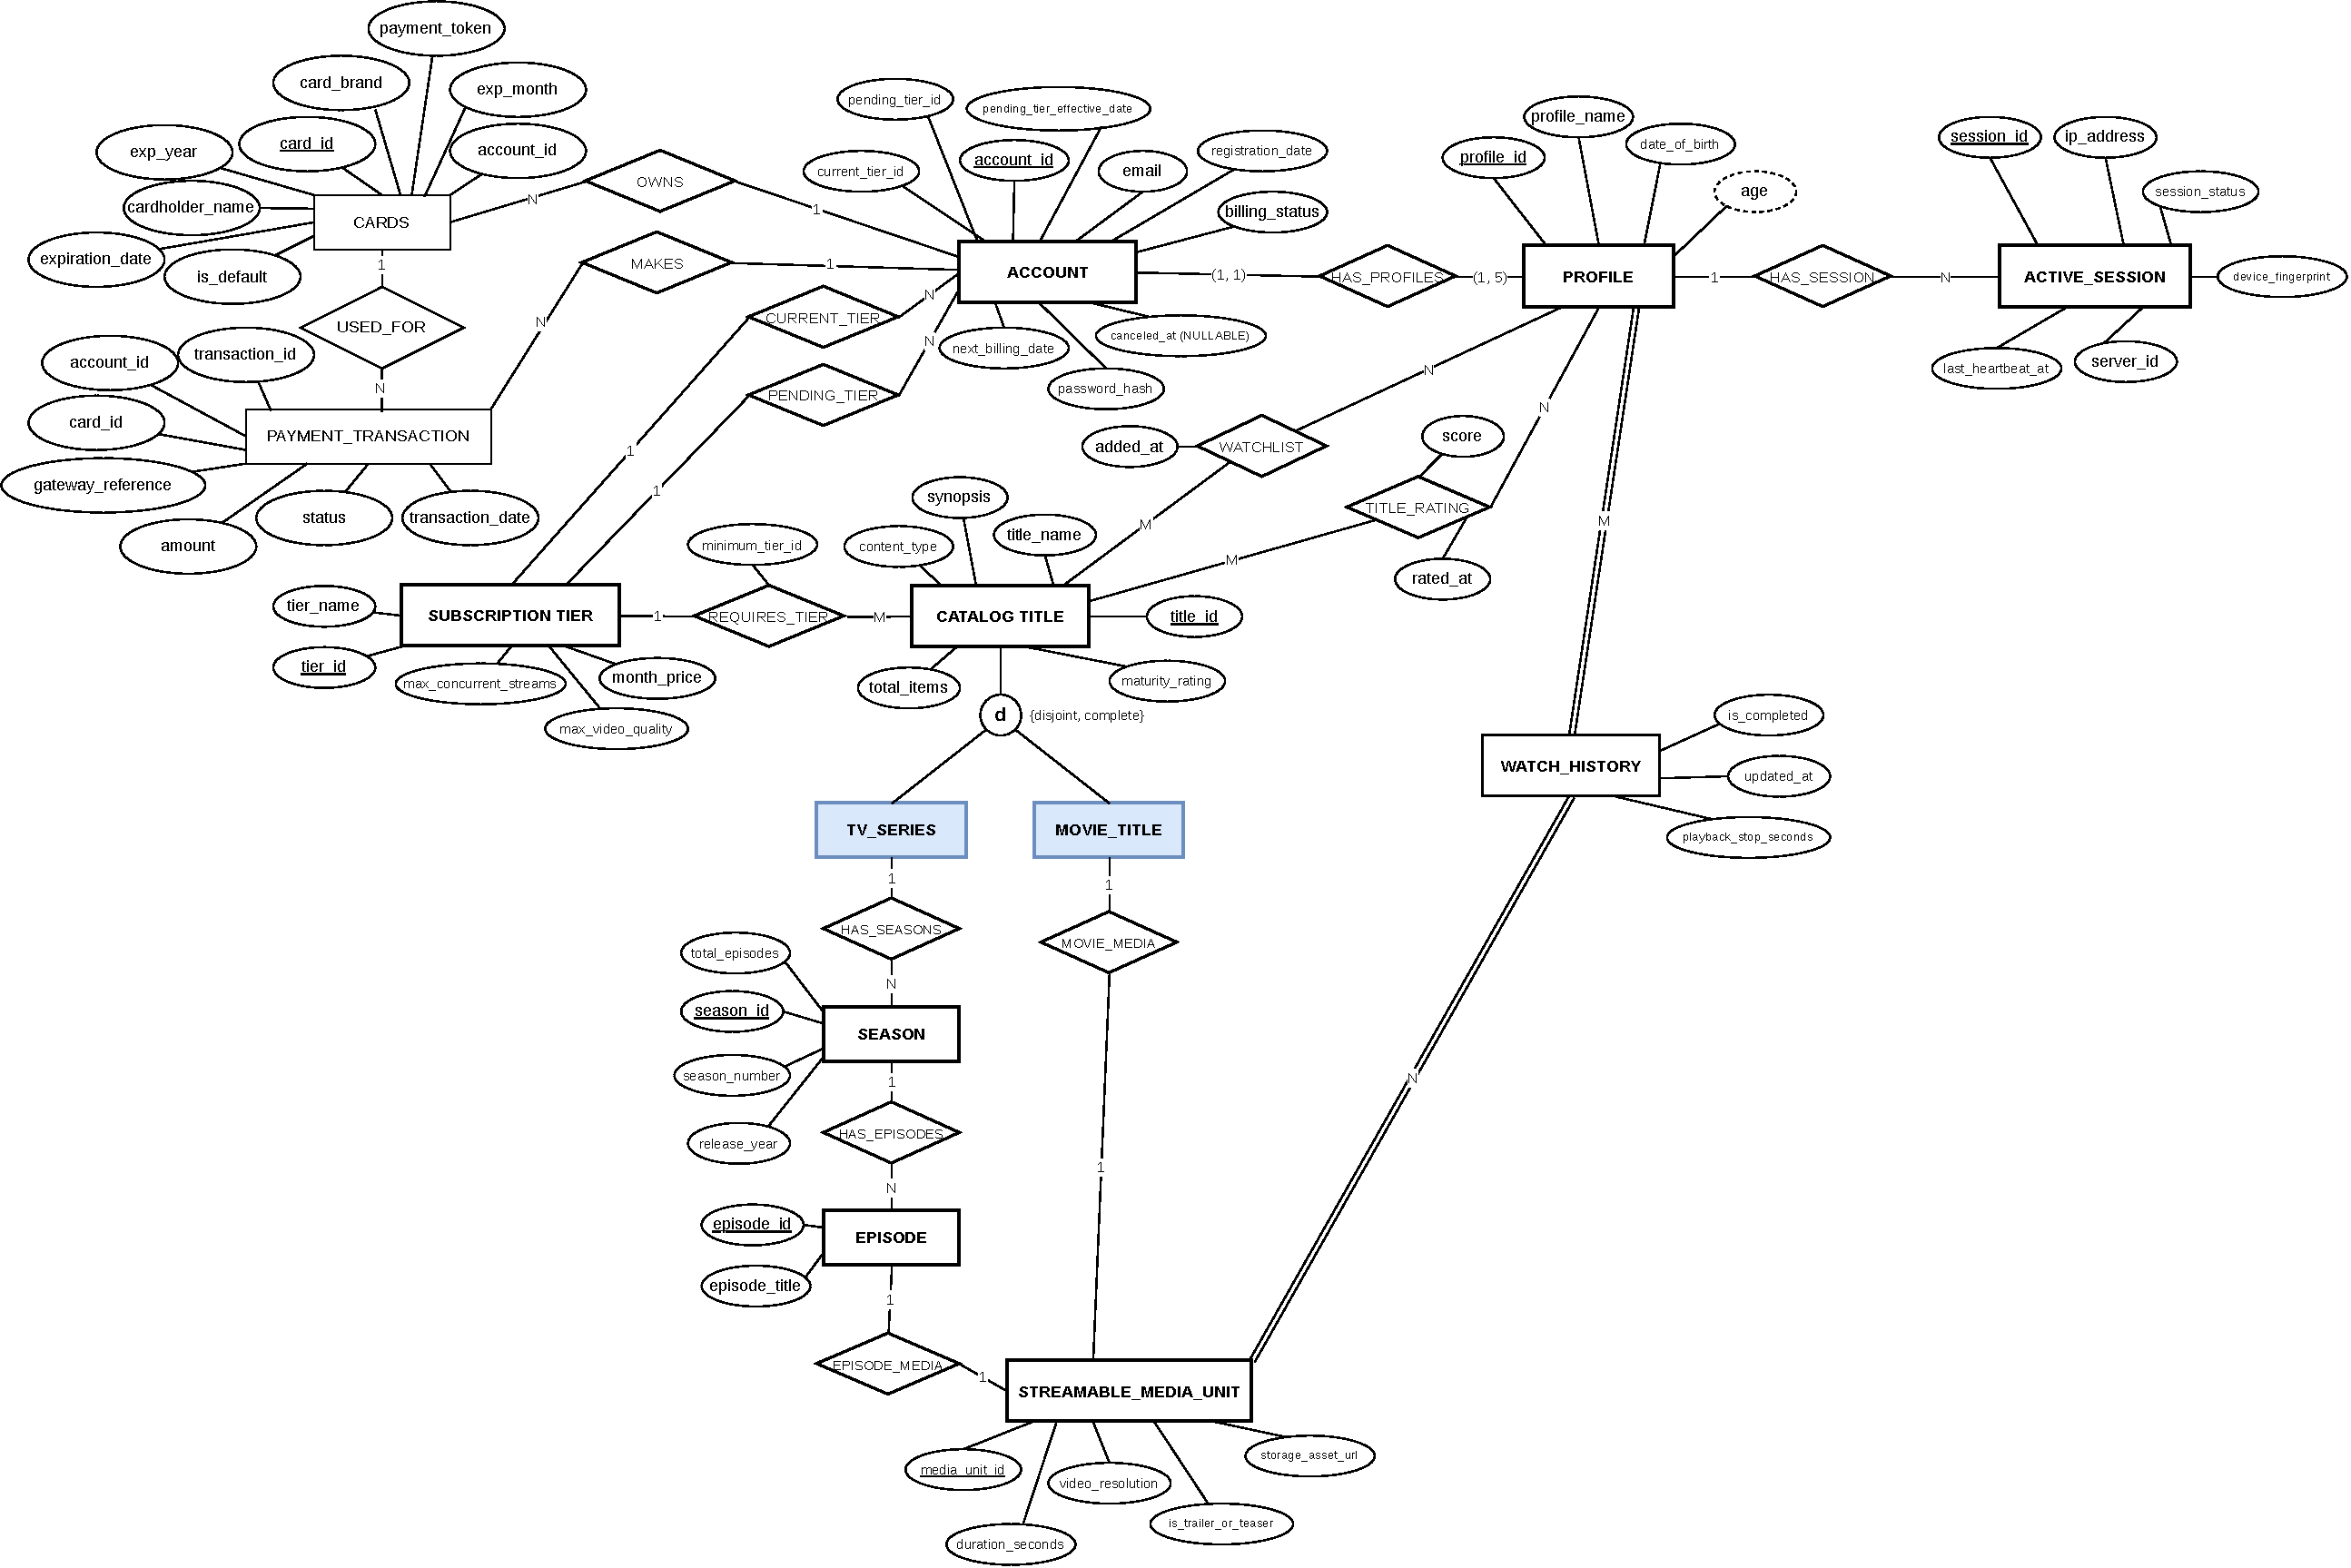
\includegraphics[width=\linewidth]{diagrams/eer.pdf}
\end{minipage}\par\medskip

\subsection*{2.2 Logical Schema Mapping}

\subsubsection*{2.2.1 Logical Relation Schema}
\begingroup\footnotesize

\subsubsection*{1. Core Platform Entities}

\begin{itemize}
\item
  \(\text{Subscription\_Tier}(\underline{\text{tier\_id}},\allowbreak   \text{tier\_name},\allowbreak   \text{monthly\_price},\allowbreak   \text{max\_concurrent\_streams},\allowbreak   \text{max\_video\_quality})\)

  \begin{itemize}
  \item
    \(\text{Candidate Key (Unique): } \{\text{tier\_name}\}\)
  \item
    \(\text{Domain Constraints: } \text{tier\_id} \in \{0,\allowbreak   1,\allowbreak   2,\allowbreak   3\}\)
  \end{itemize}
\item
  \(\text{Account}(\underline{\text{account\_id}},\allowbreak   \text{email},\allowbreak   \text{password\_hash},\allowbreak   \text{billing\_status},\allowbreak   \text{current\_tier\_id},\allowbreak   \text{pending\_tier\_id},\allowbreak   \text{pending\_tier\_effective\_date},\allowbreak   \text{registration\_date},\allowbreak   \text{next\_billing\_date},\allowbreak   \text{canceled\_at})\)

  \begin{itemize}
  \item
    \(\text{Candidate Key (Unique): } \{\text{email}\}\)
  \item
    \(\text{Foreign Keys: } \text{current\_tier\_id} \to \text{Subscription\_Tier}(\text{tier\_id}),\allowbreak   \text{pending\_tier\_id} \to \text{Subscription\_Tier}(\text{tier\_id})\)
  \end{itemize}
\item
  \(\text{Profile}(\underline{\text{profile\_id}},\allowbreak   \text{account\_id},\allowbreak   \text{profile\_name},\allowbreak   \text{is\_kids\_profile})\)

  \begin{itemize}
  \item
    \(\text{Foreign Key: } \text{account\_id} \to \text{Account}(\text{account\_id}) \text{ ON DELETE CASCADE}\)
  \item
    \(\text{Candidate Key (Unique): } \{\text{account\_id},\allowbreak   \text{profile\_name}\}\)
  \end{itemize}
\end{itemize}

\subsubsection*{2. Content \& Media Catalog (EER Specialization Mapping)}

\begin{itemize}
\item
  \(\text{Catalog\_Title}(\underline{\text{title\_id}},\allowbreak   \text{title\_name},\allowbreak   \text{synopsis},\allowbreak   \text{maturity\_rating},\allowbreak   \text{content\_type},\allowbreak   \text{minimum\_tier\_id})\)

  \begin{itemize}
  \item
    \(\text{Foreign Key: } \text{minimum\_tier\_id} \to \text{Subscription\_Tier}(\text{tier\_id})\)
  \item
    \(\text{Domain Constraints: } \text{content\_type} \in \{\text{' Movie'},\allowbreak   \text{' Series'}\},\allowbreak   \text{maturity\_rating} \in \{\text{' G'},\allowbreak   \text{' PG'},\allowbreak   \text{' PG-13'},\allowbreak   \text{' R'},\allowbreak   \text{' NC-17'}\}\)
  \end{itemize}
\item
  \(\text{Movie\_Title}(\underline{\text{title\_id}},\allowbreak   \text{media\_unit\_id})\)

  \begin{itemize}
  \item
    \(\text{Foreign Key: } \text{title\_id} \to \text{Catalog\_Title}(\text{title\_id}) \text{ ON DELETE CASCADE}\)
  \item
    \(\text{Foreign Key (Unique): } \text{media\_unit\_id} \to \text{Streamable\_Media\_Unit}(\text{media\_unit\_id})\)
  \end{itemize}
\item
  \(\text{TV\_Series}(\underline{\text{title\_id}},\allowbreak   \text{total\_seasons})\)

  \begin{itemize}
  \item
    \(\text{Foreign Key: } \text{title\_id} \to \text{Catalog\_Title}(\text{title\_id}) \text{ ON DELETE CASCADE}\)
  \end{itemize}
\item
  \(\text{Season}(\underline{\text{season\_id}},\allowbreak   \text{series\_id},\allowbreak   \text{season\_number},\allowbreak   \text{release\_year})\)

  \begin{itemize}
  \item
    \(\text{Foreign Key: } \text{series\_id} \to \text{TV\_Series}(\text{title\_id}) \text{ ON DELETE CASCADE}\)
  \item
    \(\text{Candidate Key (Unique): } \{\text{series\_id},\allowbreak   \text{season\_number}\}\)
  \end{itemize}
\item
  \(\text{Episode}(\underline{\text{episode\_id}},\allowbreak   \text{season\_id},\allowbreak   \text{media\_unit\_id},\allowbreak   \text{episode\_number},\allowbreak   \text{episode\_title})\)

  \begin{itemize}
  \item
    \(\text{Foreign Key: } \text{season\_id} \to \text{Season}(\text{season\_id}) \text{ ON DELETE CASCADE}\)
  \item
    \(\text{Foreign Key (Unique): } \text{media\_unit\_id} \to \text{Streamable\_Media\_Unit}(\text{media\_unit\_id})\)
  \item
    \(\text{Candidate Key (Unique): } \{\text{season\_id},\allowbreak   \text{episode\_number}\}\)
  \end{itemize}
\item
  \(\text{Streamable\_Media\_Unit}(\underline{\text{media\_unit\_id}},\allowbreak   \text{duration\_seconds},\allowbreak   \text{video\_resolution},\allowbreak   \text{is\_demo\_or\_trailer},\allowbreak   \text{storage\_asset\_url})\)
\end{itemize}

\subsubsection*{3. Resolved M:N Telemetry \& Associative Relations}



\begin{itemize}
\item
  \(\text{Watchlist}(\underline{\text{profile\_id}},\allowbreak   \underline{\text{title\_id}},\allowbreak   \text{added\_at})\)

  \begin{itemize}
  \item
    \(\text{Foreign Keys: } \text{profile\_id} \to \text{Profile}(\text{profile\_id}) \text{ ON DELETE CASCADE},\allowbreak   \text{title\_id} \to \text{Catalog\_Title}(\text{title\_id}) \text{ ON DELETE CASCADE}\)
  \end{itemize}
\item
  \(\text{Title\_Rating}(\underline{\text{profile\_id}},\allowbreak   \underline{\text{title\_id}},\allowbreak   \text{score},\allowbreak   \text{rated\_at})\)

  \begin{itemize}
  \item
    \(\text{Foreign Keys: } \text{profile\_id} \to \text{Profile}(\text{profile\_id}) \text{ ON DELETE CASCADE},\allowbreak   \text{title\_id} \to \text{Catalog\_Title}(\text{title\_id}) \text{ ON DELETE CASCADE}\)
  \item
    \(\text{Domain Constraint: } \text{score} \in {[}1,\allowbreak   10{]}\)
  \end{itemize}
\item
  \(\text{Watch\_History}(\underline{\text{profile\_id}},\allowbreak   \underline{\text{media\_unit\_id}},\allowbreak   \underline{\text{watched\_at}},\allowbreak   \text{playback\_stop\_seconds},\allowbreak   \text{is\_completed})\)

  \begin{itemize}
  \item
    \(\text{Foreign Keys: } \text{profile\_id} \to \text{Profile}(\text{profile\_id}) \text{ ON DELETE CASCADE},\allowbreak   \text{media\_unit\_id} \to \text{Streamable\_Media\_Unit}(\text{media\_unit\_id}) \text{ ON DELETE CASCADE}\)
  \end{itemize}
\item
  \(\text{Active\_Session}(\underline{\text{session\_id}},\allowbreak   \text{account\_id},\allowbreak   \text{profile\_id},\allowbreak   \text{ip\_address},\allowbreak   \text{device\_fingerprint},\allowbreak   \text{started\_at},\allowbreak   \text{last\_heartbeat\_at},\allowbreak   \text{session\_status})\)

  \begin{itemize}
  \item
    \(\text{Foreign Key: } (\text{account\_id},\allowbreak   \text{profile\_id}) \to \text{Profile}(\text{account\_id},\allowbreak   \text{profile\_id}) \text{ ON DELETE CASCADE}\)
  \end{itemize}
\end{itemize}

\subsubsection*{4. Billing \& Payment Infrastructure}

\par\noindent\begin{minipage}{\linewidth}\raggedright\small Credit\_\allowbreak{}Card(\underline{card\_\allowbreak{}id},\allowbreak{} account\_\allowbreak{}id,\allowbreak{} cardholder\_\allowbreak{}name,\allowbreak{} card\_\allowbreak{}brand,\allowbreak{} last\_\allowbreak{}four,\allowbreak{} exp\_\allowbreak{}month,\allowbreak{} exp\_\allowbreak{}year,\allowbreak{} payment\_\allowbreak{}token,\allowbreak{} is\_\allowbreak{}default,\allowbreak{} created\_\allowbreak{}at)\end{minipage}\par

\begin{itemize}
\item
  \textbf{Candidate Key (Unique):} \(\{ payment\_\allowbreak{} token\}\)
\item
  \textbf{Foreign Key:} \(account\_\allowbreak{} id \rightarrow Account(account\_\allowbreak{} id)\)\linebreak \texttt{ON DELETE CASCADE ON UPDATE CASCADE}
\item
  \textbf{Domain Constraints:\\
  }
\item
  \(card\_\allowbreak{} brand \in \{'VISA','MASTERCARD'\},exp\_\allowbreak{} month \in \lbrack 1,12\rbrack,exp\_\allowbreak{} year \in \lbrack 2024,2100\rbrack\)
\end{itemize}

\par\noindent\begin{minipage}{\linewidth}\raggedright\small Payment\_\allowbreak{}Transaction(\underline{transaction\_\allowbreak{}id},\allowbreak{} account\_\allowbreak{}id,\allowbreak{} card\_\allowbreak{}id,\allowbreak{} amount,\allowbreak{} currency,\allowbreak{} status,\allowbreak{} gateway\_\allowbreak{}reference,\allowbreak{} transaction\_\allowbreak{}date)\end{minipage}\par

\begin{itemize}
\item
  \textbf{Candidate Key (Unique):} \(\{ gateway\_\allowbreak{} reference\}\)
\item
  \textbf{Foreign Keys:}

  \begin{itemize}
  \item
    \(account\_\allowbreak{} id \rightarrow Account(account\_\allowbreak{} id)\)\linebreak\texttt{ON DELETE RESTRICT ON UPDATE CASCADE}
  \item
    \(card\_\allowbreak{} id \rightarrow Credit\_\allowbreak{} Card(card\_\allowbreak{} id)\)\linebreak\texttt{ON DELETE RESTRICT ON UPDATE CASCADE}
  \end{itemize}
\item
  \textbf{Domain Constraints:\\
  }
\item
  \(status \in \{'SUCCESS','FAILED','PENDING','REFUNDED'\},amount \geq 0.00\)
\end{itemize}

\endgroup
\noindent\begin{minipage}{\linewidth}
2.2.2 IE Crow\textquotesingle s Foot Schema

\par\medskip
\noindent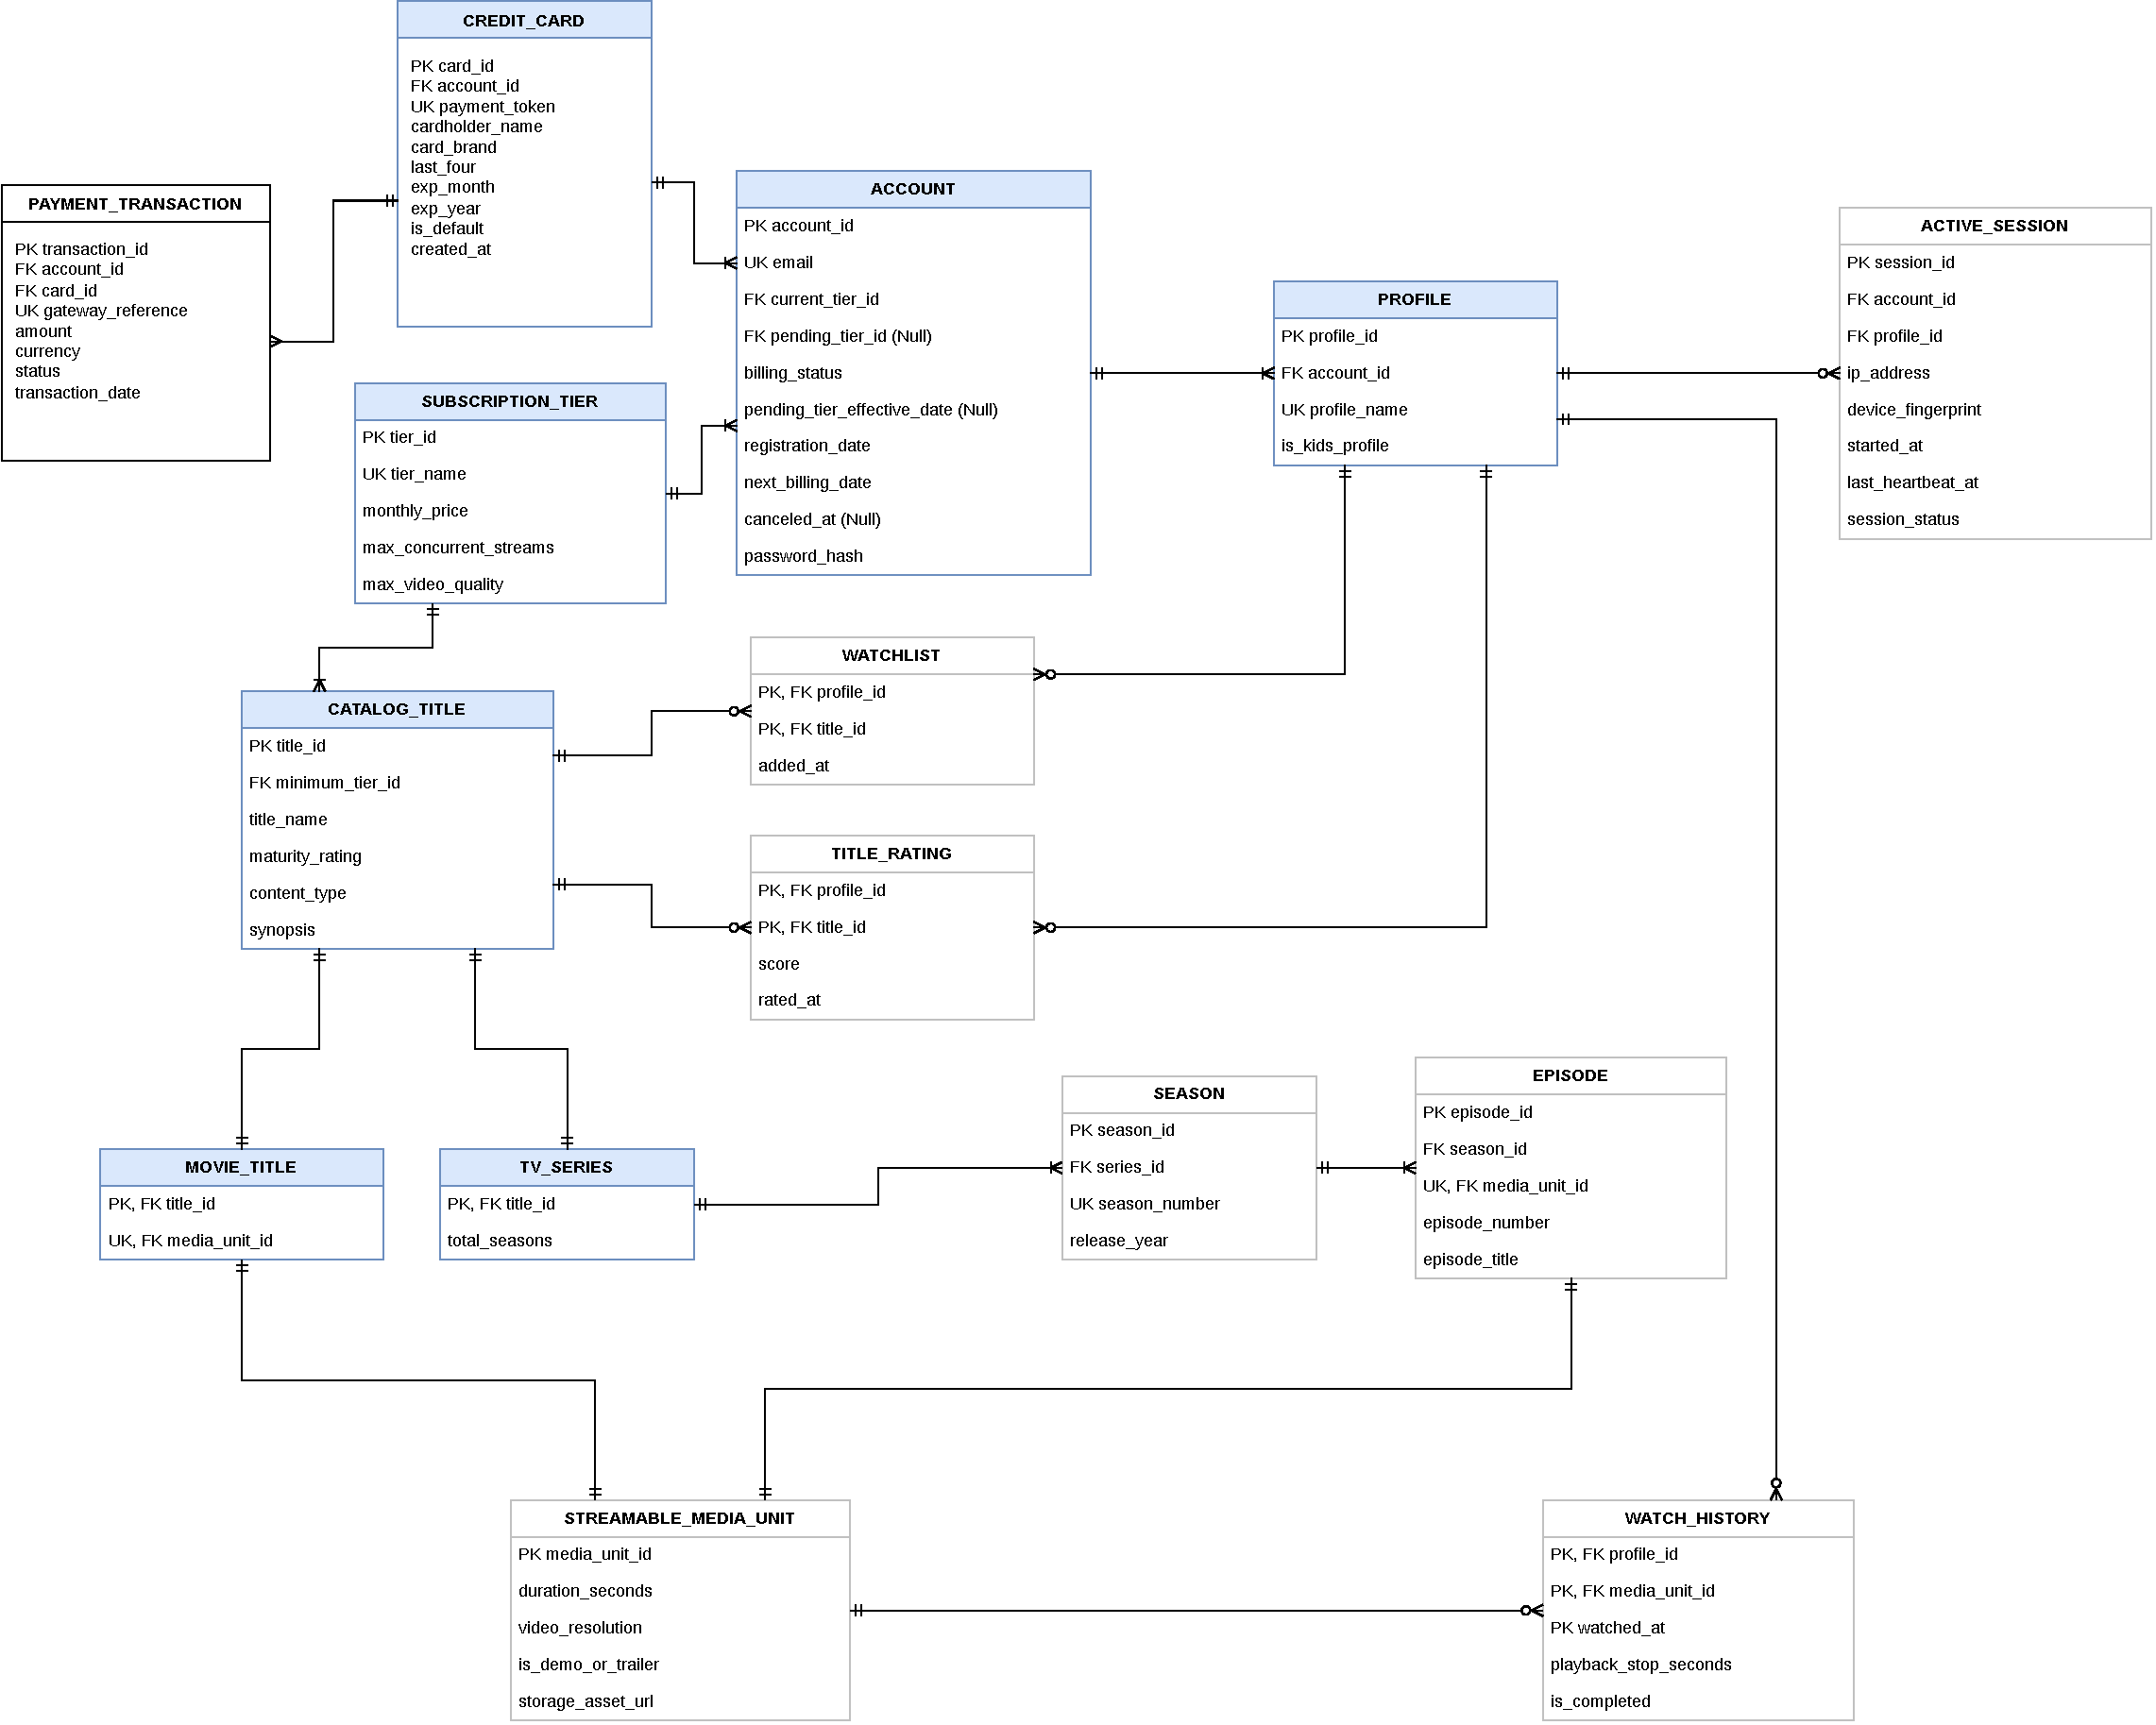
\includegraphics[width=\linewidth]{diagrams/crowfoot.pdf}
\end{minipage}
\par\medskip

\subsection*{2.3 Normalization Verification (Formal proofs for 1NF -> 3NF/BCNF)}

\subsubsection{\texorpdfstring{\textbf{2.3.1 First Normal Form (1NF) Verification}}{2.3.1 First Normal Form (1NF) Verification}}\label{first-normal-form-1nf-verification}

1. Core Platform Entities

\begin{itemize}
\item
  Subscription\_\allowbreak{}Tier \((\underline{tier\_\allowbreak{} id},tier\_\allowbreak{} name,monthly\_\allowbreak{} price,max\_\allowbreak{} concurrent\_\allowbreak{} streams,max\_\allowbreak{} video\_\allowbreak{} quality)\)

  \begin{itemize}
  \item
    Atomicity: All attributes (TINYINT, DECIMAL(6,2), VARCHAR) are scalar.
  \item
    Evaluation: Satisfies 1NF.
  \end{itemize}
\item
  Account \begin{minipage}[t]{.88\linewidth}\raggedright\small (\underline{account\_\allowbreak{}id},\allowbreak{} email,\allowbreak{} password\_\allowbreak{}hash,\allowbreak{} billing\_\allowbreak{}status,\allowbreak{} current\_\allowbreak{}tier\_\allowbreak{}id,\allowbreak{} pending\_\allowbreak{}tier\_\allowbreak{}id,\allowbreak{} pending\_\allowbreak{}tier\_\allowbreak{}effective\_\allowbreak{}date,\allowbreak{} registration\_\allowbreak{}date,\allowbreak{} next\_\allowbreak{}billing\_\allowbreak{}date,\allowbreak{} canceled\_\allowbreak{}at)\end{minipage}

  \begin{itemize}
  \item
    Atomicity: Dates, status enumerations, and foreign key references are scalar, primitive data types.
  \item
    Evaluation: Satisfies 1NF.
  \end{itemize}
\item
  Profile \((\underline{profile\_\allowbreak{} id},account\_\allowbreak{} id,profile\_\allowbreak{} name,is\_\allowbreak{} kids\_\allowbreak{} profile,date\_\allowbreak{} of\_\allowbreak{} birth)\)

  \begin{itemize}
  \item
    Atomicity: date\_\allowbreak{}of\_\allowbreak{}birth is a single scalar date rather than an unparsed composite date string. User-level settings (like language or avatar) are not crammed into comma-separated strings.
  \item
    Evaluation: Satisfies 1NF.
  \end{itemize}
\end{itemize}

\begin{itemize}
\item
  \(\mathbf{Credit\_\allowbreak{} Card}\)\textbf{:}

  \begin{itemize}
  \item
    \textbf{Atomicity:} All attributes (cardholder\_\allowbreak{}name, last\_\allowbreak{}four, exp\_\allowbreak{}month, exp\_\allowbreak{}year, payment\_\allowbreak{}token) are elementary scalar types (VARCHAR, CHAR, TINYINT, SMALLINT). Sensitive raw data (16-digit PAN, CVV) are completely excluded from the schema, avoiding multi-part composite credit card numbers.
  \item
    \textbf{Evaluation:} Satisfies 1NF.
  \end{itemize}
\item
  \(\mathbf{Payment\_\allowbreak{} Transaction}\)\textbf{:}

  \begin{itemize}
  \item
    \textbf{Atomicity:} Attributes (amount, currency, status, gateway\_\allowbreak{}reference, transaction\_\allowbreak{}date) represent single, discrete values per transaction instance. No nested arrays or repeating billing line items exist within a single transaction tuple.
  \item
    \textbf{Evaluation:} Satisfies 1NF.
  \end{itemize}
\end{itemize}

2. Content \& Media Catalog (EER Specialization)

\begin{itemize}
\item
  Catalog\_\allowbreak{}Title \((\underline{title\_\allowbreak{} id},title\_\allowbreak{} name,synopsis,maturity\_\allowbreak{} rating,content\_\allowbreak{} type,minimum\_\allowbreak{} tier\_\allowbreak{} id)\)

  \begin{itemize}
  \item
    Atomicity: All attributes represent single values.
  \item
    Design Note for Defense: Often in naive designs, designers store a multi-valued attribute like genres = "Action, Sci-Fi" directly in the title record, which commits a classic 1NF violation. Because your schema avoids storing repeated genre values in Catalog\_\allowbreak{}Title, atomicity is preserved.
  \item
    Evaluation: Satisfies 1NF.
  \end{itemize}
\item
  Movie\_\allowbreak{}Title \((\underline{title\_\allowbreak{} id},media\_\allowbreak{} unit\_\allowbreak{} id)\) \& TV\_\allowbreak{}Series \((\underline{title\_\allowbreak{} id},total\_\allowbreak{} seasons)\)

  \begin{itemize}
  \item
    Atomicity: These represent disjoint subclasses from your EER specialization (Option 8A mapping). Each stores solely its scalar attributes and foreign key.
  \item
    Evaluation: Satisfies 1NF.
  \end{itemize}
\item
  Season \((\underline{season\_\allowbreak{} id},series\_\allowbreak{} id,season\_\allowbreak{} number,release\_\allowbreak{} year)\)

  \begin{itemize}
  \item
    Atomicity: Instead of embedding an array of season numbers inside TV\_\allowbreak{}Series, the structural hierarchy is normalized into a dedicated Season relation with atomic scalar attributes. Evaluation: Satisfies 1NF.
  \end{itemize}
\end{itemize}

\subsubsection{\texorpdfstring{\textbf{2.3.2 Second Normal Form (2NF) Verification}}{2.3.2 Second Normal Form (2NF) Verification}}\label{second-normal-form-2nf-verification}

\emph{Prime vs. non-prime attributes are evaluated with respect to all candidate keys declared in the data dictionary of §3.}

A partial dependency can only exist if a key contains two or more attributes (a composite key). A single-column key cannot have a non-empty proper subset.

Because of this rule, 10 out of 13 tables are in 2NF by definition:

\begin{itemize}
\item
  Subscription\_\allowbreak{}Tier (\(\underline{tier\_\allowbreak{} id}\))
\item
  Account (\(\underline{account\_\allowbreak{} id}\))
\item
  Profile (\(\underline{profile\_\allowbreak{} id}\))
\item
  Catalog\_\allowbreak{}Title (\(\underline{title\_\allowbreak{} id}\))
\item
  Movie\_\allowbreak{}Title (\(\underline{title\_\allowbreak{} id}\))
\item
  TV\_\allowbreak{}Series (\(\underline{title\_\allowbreak{} id}\))
\item
  Season (\(\underline{season\_\allowbreak{} id}\))
\item
  Episode (\(\underline{episode\_\allowbreak{} id}\))
\item
  Streamable\_\allowbreak{}Media\_\allowbreak{}Unit (\(\underline{media\_\allowbreak{} unit\_\allowbreak{} id}\))
\item
  Active\_\allowbreak{}Session (\(\underline{session\_\allowbreak{} id}\))
\end{itemize}

1. Watchlist

\begin{itemize}
\item
  Primary Key: \{profile\_\allowbreak{}id,title\_\allowbreak{}id\}
\item
  Non-prime Attribute: added\_\allowbreak{}at
\item
  Dependency Analysis:
\end{itemize}

\begin{itemize}
\item
  \({\text{profile\_id}} \not\to \text{added\_at}\) (A profile bookmarks many titles at different times)
\item
  \({\text{title\_id}} \not\to \text{added\_at}\) (A title is bookmarked by different profiles at different times)
\item
    \({\text{profile\_id, title\_id}} \not\to \text{added\_at}\) (The timestamp records the exact event of this profile saving this title)
\end{itemize}

\begin{itemize}
\item
  Verdict: added\_\allowbreak{}at is fully functionally dependent on the whole primary key. Satisfies 2NF.
\end{itemize}

2. Title\_\allowbreak{}Rating

\begin{itemize}
\item
  Primary Key: \{profile\_\allowbreak{}id,title\_\allowbreak{}id\}
\item
  Non-prime Attributes: score, rated\_\allowbreak{}at
\item
  Dependency Analysis:
\end{itemize}

\begin{itemize}
\item
  \({\text{profile\_id}} \not\to \text{score}\) (A user gives different scores to different movies)
\item
  \({\text{title\_id}} \not\to \text{score}\) (A movie receives different scores from different users)
\item
  Neither score nor rated\_\allowbreak{}at can be determined by a single component of the key. Both require the combination \{profile\_\allowbreak{}id,title\_\allowbreak{}id\}.
\end{itemize}

\begin{itemize}
\item
  Verdict: Fully functionally dependent. No partial dependency exists. Satisfies 2NF.
\end{itemize}

3. Watch\_\allowbreak{}History

\subsubsection{Primary Key: \{profile\_\allowbreak{}id,media\_\allowbreak{}unit\_\allowbreak{}id,watched\_\allowbreak{}at\}}\label{primary-key-profile_idmedia_unit_idwatched_at}

\subsubsection{Non-prime Attributes: playback\_\allowbreak{}stop\_\allowbreak{}seconds, is\_\allowbreak{}completed}\label{non-prime-attributes-playback_stop_seconds-is_completed}

\subsubsection{Dependency Analysis:}\label{dependency-analysis}

\subsubsection{Does a single profile or media unit alone determine the stop position? No.}\label{does-a-single-profile-or-media-unit-alone-determine-the-stop-position-no.}

\subsubsection{Does \{profile\_\allowbreak{}id,media\_\allowbreak{}unit\_\allowbreak{}id\}playback\_\allowbreak{}stop\_\allowbreak{}seconds? If a user watches the same media unit on multiple separate occasions (tracked by the discriminator watched\_\allowbreak{}at), each viewing session has its own progress checkpoint and completion flag.}\label{does-profile_idmedia_unit_idplayback_stop_seconds-if-a-user-watches-the-same-media-unit-on-multiple-separate-occasions-tracked-by-the-discriminator-watched_at-each-viewing-session-has-its-own-progress-checkpoint-and-completion-flag.}

\subsubsection{Both playback\_\allowbreak{}stop\_\allowbreak{}seconds and is\_\allowbreak{}completed describe that specific viewing instance identified by the triplet \{profile\_\allowbreak{}id,media\_\allowbreak{}unit\_\allowbreak{}id,watched\_\allowbreak{}at\}.}\label{both-playback_stop_seconds-and-is_completed-describe-that-specific-viewing-instance-identified-by-the-triplet-profile_idmedia_unit_idwatched_at.}

\subsubsection{Verdict: Fully functionally dependent. Satisfies 2NF.}\label{verdict-fully-functionally-dependent.-satisfies-2nf.}

\subsubsection{}\label{section}

\begin{itemize}
\item
  \(\mathbf{Credit\_\allowbreak{} Card}\)\textbf{:}

  \begin{itemize}
  \item
    Primary Key: \(\{ card\_\allowbreak{} id\}\) (single attribute).
  \item
    Alternate Candidate Key: \(\{ payment\_\allowbreak{} token\}\) (single attribute).
  \item
    Because every candidate key consists of a single attribute, no proper subset of a key can exist. Therefore, partial dependencies are mathematically impossible.
  \item
    \textbf{Verdict:} Satisfies 2NF by definition.
  \end{itemize}
\item
  \(\mathbf{Payment\_\allowbreak{} Transaction}\)\textbf{:}

  \begin{itemize}
  \item
    Primary Key: \(\{ transaction\_\allowbreak{} id\}\) (single attribute).
  \item
    Alternate Candidate Key: \(\{ gateway\_\allowbreak{} reference\}\) (single attribute).
  \item
    Similar to \(Credit\_\allowbreak{} Card\), all candidate keys are atomic single-attribute keys.
  \end{itemize}
\end{itemize}

\subsubsection{\texorpdfstring{\textbf{Verdict:} Satisfies 2NF by definition.\\
\textbf{2.3.3 Boyce-Codd Normal Form (BCNF)} }{Verdict: Satisfies 2NF by definition. 2.3.3 Boyce-Codd Normal Form (BCNF) }}\label{verdict-satisfies-2nf-by-definition.-2.3.3-boyce-codd-normal-form-bcnf}

\paragraph{Category A: Relations with a Single Candidate Key}\label{category-a-relations-with-a-single-candidate-key}

When a relation has only one candidate key (which is chosen as the Primary Key) and is already in 3NF, it is guaranteed to be in BCNF. In these tables, no non-key attribute determines any other attribute:

\begin{itemize}
\item
  Profile: \(profile\_\allowbreak{} id \rightarrow \{ account\_\allowbreak{} id,profile\_\allowbreak{} name,is\_\allowbreak{} kids\_\allowbreak{} profile,date\_\allowbreak{} of\_\allowbreak{} birth\}\)
\item
  Catalog\_\allowbreak{}Title: \(title\_\allowbreak{} id \rightarrow \{ title\_\allowbreak{} name,synopsis,maturity\_\allowbreak{} rating,content\_\allowbreak{} type,minimum\_\allowbreak{} tier\_\allowbreak{} id\}\)
\item
  TV\_\allowbreak{}Series: \(title\_\allowbreak{} id \rightarrow \{ total\_\allowbreak{} seasons\}\)
\item
  \textbf{Active\_Session:} \texttt{session\_id} $\rightarrow$ \{\texttt{account\_id}, \texttt{profile\_id}, \texttt{ip\_address}, \texttt{device\_fingerprint}, \texttt{started\_at}, \texttt{last\_heartbeat\_at}, \texttt{session\_status}\}
\item
  Active\_\allowbreak{}Session:\\
  \[\begin{aligned} session_{i}d \rightarrow account_{i}d,profile_{i}d,\\ &ip_{a}ddress,device_{f}ingerprint,\\ &started_{a}t,last_{h}eartbeat_{a}t,session_{s}tatus \end{aligned}\]
\item
  Watchlist: \(\{ profile\_\allowbreak{} id,title\_\allowbreak{} id\} \rightarrow \{ added\_\allowbreak{} at\}\)
\item
  Title\_\allowbreak{}Rating: \(\{ profile\_\allowbreak{} id,title\_\allowbreak{} id\} \rightarrow \{ score,rated\_\allowbreak{} at\}\)
\item
  Watch\_\allowbreak{}History: \(\{ profile\_\allowbreak{} id,media\_\allowbreak{} unit\_\allowbreak{} id,watched\_\allowbreak{} at\} \rightarrow \{ playback\_\allowbreak{} stop\_\allowbreak{} seconds,is\_\allowbreak{} completed\}\)
\end{itemize}

In all of the above, the left-hand side (\(X\)) is the Primary Key (a superkey). Therefore, each satisfies BCNF.

\paragraph{Category B: Relations with Multiple Candidate / Overlapping Keys}\label{category-b-relations-with-multiple-candidate-overlapping-keys}

BCNF primarily exists to catch edge-case anomalies in tables with multiple overlapping candidate keys. Let's evaluate the relations in your schema that have alternate candidate keys:

1. Subscription\_\allowbreak{}Tier

\begin{itemize}
\item
  Candidate Keys: \(K_{1} = \{ tier\_\allowbreak{} id\}\), \(K_{2} = \{ tier\_\allowbreak{} name\}\)
\item
  Dependencies:

  \begin{itemize}
  \item
    \(tier\_\allowbreak{} id \rightarrow \{ tier\_\allowbreak{} name,monthly\_\allowbreak{} price,max\_\allowbreak{} concurrent\_\allowbreak{} streams,max\_\allowbreak{} video\_\allowbreak{} quality\}\)
  \item
    \(tier\_\allowbreak{} name \rightarrow \{ tier\_\allowbreak{} id,monthly\_\allowbreak{} price,max\_\allowbreak{} concurrent\_\allowbreak{} streams,max\_\allowbreak{} video\_\allowbreak{} quality\}\)
  \end{itemize}
\item
  Determinant Check: Both \(tier\_\allowbreak{} id\) and \(tier\_\allowbreak{} name\) are candidate keys (superkeys). Satisfies BCNF.
\end{itemize}

2. Account

\begin{itemize}
\item
  Candidate Keys: \(K_{1} = \{ account\_\allowbreak{} id\}\), \(K_{2} = \{ email\}\)
\item
  Dependencies:

  \begin{itemize}
  \item
    \(\text{account\_id} \to {\text{email},\allowbreak  \text{password\_hash},\allowbreak  \text{billing\_status},\allowbreak  \dots}\)
  \item
    \(\text{email} \to {\text{account\_id},\allowbreak  \text{password\_hash},\allowbreak  \text{billing\_status},\allowbreak  \dots}\)
  \end{itemize}
\item
  Determinant Check: Both determinants are candidate keys (superkeys). Foreign keys like \(current\_\allowbreak{} tier\_\allowbreak{} id\) or \(pending\_\allowbreak{} tier\_\allowbreak{} id\) do not determine other non-key attributes within this table. Satisfies BCNF.
\end{itemize}

3. Movie\_\allowbreak{}Title (1:1 Specialization Junction)

\begin{itemize}
\item
  Candidate Keys: \(K_{1} = \{ title\_\allowbreak{} id\}\), \(K_{2} = \{ media\_\allowbreak{} unit\_\allowbreak{} id\}\)
\item
  Dependencies:

  \begin{itemize}
  \item
    \(title\_\allowbreak{} id \rightarrow media\_\allowbreak{} unit\_\allowbreak{} id\)
  \item
    \(media\_\allowbreak{} unit\_\allowbreak{} id \rightarrow title\_\allowbreak{} id\)
  \end{itemize}
\item
  Determinant Check: Both are superkeys. Satisfies BCNF.
\end{itemize}

4. Season

\begin{itemize}
\item
  Candidate Keys: \(K_{1} = \{ season\_\allowbreak{} id\}\), \(K_{2} = \{ series\_\allowbreak{} id,season\_\allowbreak{} number\}\)
\item
  Dependencies:

  \begin{itemize}
  \item
    \(season\_\allowbreak{} id \rightarrow \{ series\_\allowbreak{} id,season\_\allowbreak{} number,release\_\allowbreak{} year\}\)
  \item
    \(\{ series\_\allowbreak{} id,season\_\allowbreak{} number\} \rightarrow \{ season\_\allowbreak{} id,release\_\allowbreak{} year\}\)
  \end{itemize}
\item
  Determinant Check: Neither \(series\_\allowbreak{} id\) nor \(season\_\allowbreak{} number\) alone determines \(release\_\allowbreak{} year\). The only determinants are the two candidate keys. Both are superkeys. Satisfies BCNF.
\end{itemize}

5. Episode

\begin{itemize}
\item
  Candidate Keys:

  \begin{itemize}
  \item
    \(K_{1} = \{ episode\_\allowbreak{} id\}\)
  \item
    \(K_{2} = \{ media\_\allowbreak{} unit\_\allowbreak{} id\}\) (each episode has exactly one unique playable stream)
  \item
    \(K_{3} = \{ season\_\allowbreak{} id,episode\_\allowbreak{} number\}\)
  \end{itemize}
\item
  Dependencies: Every non-trivial dependency has \(K_{1}\), \(K_{2}\), or \(K_{3}\) as its determinant. Since each determinant is a candidate key, it satisfies BCNF.
\end{itemize}

\subparagraph{\texorpdfstring{\textbf{6. Cards}}{6. Cards}}\label{cards}

\begin{itemize}
\item
  \textbf{Candidate Keys:} \(K_{1} = \{ card\_\allowbreak{} id\},K_{2} = \{ payment\_\allowbreak{} token\}\)
\item
  \textbf{Functional Dependencies:}

  \begin{itemize}
  \item
    \begin{minipage}[t]{.88\linewidth}\raggedright\small FD\_\allowbreak{}\{1\}:\{card\_\allowbreak{}id\}\(\rightarrow\) \{account\_\allowbreak{}id,\allowbreak{} cardholder\_\allowbreak{}name,\allowbreak{} card\_\allowbreak{}brand,\allowbreak{} last\_\allowbreak{}four,\allowbreak{} exp\_\allowbreak{}month,\allowbreak{} exp\_\allowbreak{}year,\allowbreak{} payment\_\allowbreak{}token,\allowbreak{} is\_\allowbreak{}default,\allowbreak{} created\_\allowbreak{}at\}\end{minipage}
  \item
    \begin{minipage}[t]{.88\linewidth}\raggedright\small FD\_\allowbreak{}\{2\}:\{payment\_\allowbreak{}token\}\(\rightarrow\) \{card\_\allowbreak{}id,\allowbreak{} account\_\allowbreak{}id,\allowbreak{} cardholder\_\allowbreak{}name,\allowbreak{} card\_\allowbreak{}brand,\allowbreak{} last\_\allowbreak{}four,\allowbreak{} exp\_\allowbreak{}month,\allowbreak{} exp\_\allowbreak{}year,\allowbreak{} is\_\allowbreak{}default,\allowbreak{} created\_\allowbreak{}at\}\end{minipage}
  \end{itemize}
\item
  \textbf{Determinant Check:}

  \begin{itemize}
  \item
    For \(FD_{1}\), the determinant \(\{ card\_\allowbreak{} id\}\) is candidate key \(K_{1}\) (a superkey).
  \item
    For \(FD_{2}\), the determinant \(\{ payment\_\allowbreak{} token\}\) is candidate key \(K_{2}\) (a superkey).
  \item
    Attributes such as \(account\_\allowbreak{} id\) or \(last\_\allowbreak{} four\) do not uniquely determine any other attributes (an account may hold multiple cards, and multiple users can share the same last four digits).
  \end{itemize}
\item
  \textbf{Verdict:} Every determinant is a superkey. \textbf{Satisfies BCNF.}
\end{itemize}

\subparagraph{\texorpdfstring{\textbf{7.} \(\mathbf{Payment\_\allowbreak{} Transaction}\)}{7. \mathbf\{Payment\_\allowbreak{} Transaction\}}}\label{mathbfpayment_-transaction}

\begin{itemize}
\item
  \textbf{Candidate Keys:} \(K_{1} = \{ transaction\_\allowbreak{} id\},K_{2} = \{ gateway\_\allowbreak{} reference\}\)
\item
  \textbf{Functional Dependencies:}

  \begin{itemize}
  \item
    \(FD_{1}:\{ transaction\_\allowbreak{} id\} \rightarrow \{ account\_\allowbreak{} id,card\_\allowbreak{} id,amount,currency,status,gateway\_\allowbreak{} reference,transaction\_\allowbreak{} date\}\)
  \item
    \(FD_{2}:\{ gateway\_\allowbreak{} reference\} \rightarrow \{ transaction\_\allowbreak{} id,account\_\allowbreak{} id,card\_\allowbreak{} id,amount,currency,status,transaction\_\allowbreak{} date\}\)
  \end{itemize}
\item
  \textbf{Determinant Check:}

  \begin{itemize}
  \item
    For \(FD_{1}\), the determinant is \(K_{1}\) (a superkey).
  \item
    For \(FD_{2}\), the determinant is \(K_{2}\) (a superkey).
  \item
    Foreign keys \(account\_\allowbreak{} id\) and \(card\_\allowbreak{} id\) participate in \(1:N\) relationships and cannot functionally determine transaction status, amounts, or timestamps independently.
  \end{itemize}
\item
  \textbf{Verdict:} Every determinant is a superkey. \textbf{Satisfies BCNF.}
\end{itemize}

\section*{3. Data Dictionary (Adapted from ISO/IEC 11179)}

\subsection*{3.1 Core Platform \& Membership Entities}

\subsubsection*{Table 3.1.1: Subscription\_\allowbreak{}Tier}
\emph{Defines service tier definitions, pricing, concurrent stream caps, and maximum streaming resolution.}

{\def\LTcaptype{none}
\begin{longtable}[]{@{}
  >{\raggedright\arraybackslash}p{(\linewidth - 10\tabcolsep) * \real{0.20}}
  >{\raggedright\arraybackslash}p{(\linewidth - 10\tabcolsep) * \real{0.16}}
  >{\raggedright\arraybackslash}p{(\linewidth - 10\tabcolsep) * \real{0.10}}
  >{\raggedright\arraybackslash}p{(\linewidth - 10\tabcolsep) * \real{0.11}}
  >{\raggedright\arraybackslash}p{(\linewidth - 10\tabcolsep) * \real{0.13}}
  >{\raggedright\arraybackslash}p{(\linewidth - 10\tabcolsep) * \real{0.30}}@{}}
\arrayrulecolor{black}\toprule
\textbf{Attribute Name} & \textbf{Data Type} & \textbf{Key Type} & \textbf{Nullable?} & \textbf{Default Value} & \textbf{Business Rules / Constraints} \\
\midrule
\endhead
\bottomrule
\endlastfoot
tier\_\allowbreak{}id & TINYINT UNSIGNED & PK & No & None & Surrogate primary key. Domain constraint: $\in \{0,1,2,3\}$ ($0 = \text{Free/Guest}$, $1 = \text{Basic}$, $2 = \text{Standard}$, $3 = \text{Premium}$). \\
\arrayrulecolor{black!20}\midrule
tier\_\allowbreak{}name & VARCHAR(20) & AK & No & None & Unique tier name (UNIQUE). Restricted to: 'Free', 'Basic', 'Standard', 'Premium'. \\
\arrayrulecolor{black!20}\midrule
monthly\_\allowbreak{}price & DECIMAL(6,2) & None & No & 0.00 & Monthly recurring subscription charge in USD. Must satisfy $\ge 0.00$. Fixed at 0.00 for tier\_\allowbreak{}id = 0. \\
\arrayrulecolor{black!20}\midrule
max\_\allowbreak{}concurrent\_\allowbreak{}streams & TINYINT UNSIGNED & None & No & 1 & Max active streaming sessions allowed concurrently across the account ($1 \le n \le 10$). \\
\arrayrulecolor{black!20}\midrule
max\_\allowbreak{}video\_\allowbreak{}quality & VARCHAR(10) & None & No & '480p' & Maximum stream resolution permitted: '480p', '720p', '1080p', '4K UHD'. \\
\arrayrulecolor{black}
\end{longtable}
}

\subsubsection*{Table 3.1.2: Account}

\emph{Master billing account entity responsible for subscription ownership and administrative privileges.}

{\def\LTcaptype{none} % do not increment counter
\begin{longtable}[]{@{}
  >{\raggedright\arraybackslash}p{(\linewidth - 10\tabcolsep) * \real{0.20}}
  >{\raggedright\arraybackslash}p{(\linewidth - 10\tabcolsep) * \real{0.16}}
  >{\raggedright\arraybackslash}p{(\linewidth - 10\tabcolsep) * \real{0.10}}
  >{\raggedright\arraybackslash}p{(\linewidth - 10\tabcolsep) * \real{0.11}}
  >{\raggedright\arraybackslash}p{(\linewidth - 10\tabcolsep) * \real{0.13}}
  >{\raggedright\arraybackslash}p{(\linewidth - 10\tabcolsep) * \real{0.30}}@{}}
\arrayrulecolor{black}\toprule\noalign{}
\endhead
\bottomrule\noalign{}
\endlastfoot
\textbf{Attribute Name} & \textbf{Data Type} & \textbf{Key Type} & \textbf{Nullable?} & \textbf{Default Value} & \textbf{Business Rules / Constraints} \\ 
\midrule
account\_\allowbreak{}id & INT UNSIGNED & PK & No & None & Auto-incrementing surrogate primary key identifying the customer account. \\ \arrayrulecolor{black!20}\midrule
email & VARCHAR(255) & AK & No & None & Unique login credential (UNIQUE). Must satisfy standard RFC 5322 email regex pattern. \\ \arrayrulecolor{black!20}\midrule
password\_\allowbreak{}hash & CHAR(60) & None & No & None & Cryptographic password digest generated via bcrypt/Argon2. Fixed length of 60 characters. \\ \arrayrulecolor{black!20}\midrule
billing\_\allowbreak{}status & VARCHAR(20) & None & No & \textquotesingle Active\textquotesingle{} & Domain constraint: CHECK (billing\_\allowbreak{}status IN (\textquotesingle Active\textquotesingle, \textquotesingle Past\_\allowbreak{}Due\textquotesingle, \textquotesingle Suspended\textquotesingle, \textquotesingle Inactive\textquotesingle)). \\ \arrayrulecolor{black!20}\midrule
current\_\allowbreak{}tier\_\allowbreak{}id & TINYINT UNSIGNED & FK & No & 0 & References Subscription\_\allowbreak{}Tier(tier\_\allowbreak{}id) ON DELETE RESTRICT ON UPDATE CASCADE. Defaults to 0 (Free tier) upon account registration (\textbf{BR-10}); upgrading to tier\_\allowbreak{}id \textgreater{} 0 requires a saved Credit\_\allowbreak{}Card (\textbf{BR-11}). \\ \arrayrulecolor{black!20}\midrule
pending\_\allowbreak{}tier\_\allowbreak{}id & TINYINT UNSIGNED & FK & Yes & NULL & References Subscription\_\allowbreak{}Tier(tier\_\allowbreak{}id) ON DELETE SET NULL ON UPDATE CASCADE. Stores scheduled downgrade tier (BR-14). \\ \arrayrulecolor{black!20}\midrule
pending\_\allowbreak{}tier\_\allowbreak{}effective\_\allowbreak{}date & DATE & None & Yes & NULL & Effective start date of pending subscription change. Must satisfy \(\geq registration\_\allowbreak{} date\). \\ \arrayrulecolor{black!20}\midrule
registration\_\allowbreak{}date & DATE & None & No & (CURRENT\_\allowbreak{}DATE) & Calendar date when the account was initially created. \\ \arrayrulecolor{black!20}\midrule
next\_\allowbreak{}billing\_\allowbreak{}date & DATE & None & No & None & Date of upcoming 30-day recurring charge (BR-12). Must satisfy \(> registration\_\allowbreak{} date\). \\ \arrayrulecolor{black!20}\midrule
canceled\_\allowbreak{}at & TIMESTAMP & None & Yes & NULL & Timestamp of subscription cancellation. Triggers the 10-month data retention grace period (BR-15). \\
\end{longtable}
}

\paragraph{Table 3.1.3: Profile}\label{table-3.1.3-profile}

\emph{Viewer partition entity isolated under a parent Account. Enforces viewing boundaries and parental controls.}

{\def\LTcaptype{none} % do not increment counter
\begin{longtable}[]{@{}
  >{\raggedright\arraybackslash}p{(\linewidth - 10\tabcolsep) * \real{0.20}}
  >{\raggedright\arraybackslash}p{(\linewidth - 10\tabcolsep) * \real{0.16}}
  >{\raggedright\arraybackslash}p{(\linewidth - 10\tabcolsep) * \real{0.10}}
  >{\raggedright\arraybackslash}p{(\linewidth - 10\tabcolsep) * \real{0.11}}
  >{\raggedright\arraybackslash}p{(\linewidth - 10\tabcolsep) * \real{0.13}}
  >{\raggedright\arraybackslash}p{(\linewidth - 10\tabcolsep) * \real{0.30}}@{}}
\arrayrulecolor{black}\toprule\noalign{}
\endhead
\bottomrule\noalign{}
\endlastfoot
\textbf{Attribute Name} & \textbf{Data Type} & \textbf{Key Type} & \textbf{Nullable?} & \textbf{Default Value} & \textbf{Business Rules / Constraints} \\ 
\midrule
profile\_\allowbreak{}id & INT UNSIGNED & PK & No & None & Auto-incrementing unique identifier for each viewer partition. \\ \arrayrulecolor{black!20}\midrule
account\_\allowbreak{}id & INT UNSIGNED & FK & No & None & References Account(account\_\allowbreak{}id) ON DELETE CASCADE ON UPDATE CASCADE (BR-06). \\ \arrayrulecolor{black!20}\midrule
profile\_\allowbreak{}name & VARCHAR(30) & None & No & None & Display moniker. Composite Candidate Key: UNIQUE(account\_\allowbreak{}id, profile\_\allowbreak{}name). \\ \arrayrulecolor{black!20}\midrule
is\_\allowbreak{}kids\_\allowbreak{}profile & BOOLEAN & None & No & FALSE & Parental control flag. If TRUE, access is restricted from \textquotesingle R\textquotesingle{} and \textquotesingle TV-MA\textquotesingle{} content (BR-04). \\ \arrayrulecolor{black!20}\midrule
date\_\allowbreak{}of\_\allowbreak{}birth & DATE & None & Yes & NULL & Viewer birth date. Used to compute dynamic derived age: \((CURRENT\_\allowbreak{} DATE - date\_\allowbreak{} of\_\allowbreak{} birth)\). \\
\end{longtable}
}

\subsubsection{3.2 Content Catalog, EER Hierarchy \& Media Units}\label{content-catalog-eer-hierarchy-media-units}

\paragraph{Table 3.2.1: Catalog\_\allowbreak{}Title (EER Superclass)}\label{table-3.2.1-catalog_title-eer-superclass}

\emph{High-level abstract media catalog container for all browsable, discoverable entertainment assets.}

{\def\LTcaptype{none} % do not increment counter
\begin{longtable}[]{@{}
  >{\raggedright\arraybackslash}p{(\linewidth - 10\tabcolsep) * \real{0.20}}
  >{\raggedright\arraybackslash}p{(\linewidth - 10\tabcolsep) * \real{0.16}}
  >{\raggedright\arraybackslash}p{(\linewidth - 10\tabcolsep) * \real{0.10}}
  >{\raggedright\arraybackslash}p{(\linewidth - 10\tabcolsep) * \real{0.11}}
  >{\raggedright\arraybackslash}p{(\linewidth - 10\tabcolsep) * \real{0.13}}
  >{\raggedright\arraybackslash}p{(\linewidth - 10\tabcolsep) * \real{0.30}}@{}}
\arrayrulecolor{black}\toprule\noalign{}
\endhead
\bottomrule\noalign{}
\endlastfoot
\textbf{Attribute Name} & \textbf{Data Type} & \textbf{Key Type} & \textbf{Nullable?} & \textbf{Default Value} & \textbf{Business Rules / Constraints} \\ \arrayrulecolor{black}\midrule
title\_\allowbreak{}id & INT UNSIGNED & PK & No & None & Unique surrogate primary key identifying each catalog entry. \\ \arrayrulecolor{black!20}\midrule
title\_\allowbreak{}name & VARCHAR(150) & None & No & None & Official public display name of the title. Cannot be blank or empty string. \\ \arrayrulecolor{black!20}\midrule
synopsis & TEXT & None & Yes & NULL & Descriptive narrative summary and storyline overview. \\ \arrayrulecolor{black!20}\midrule
maturity\_\allowbreak{}rating & VARCHAR(10) & None & No & \textquotesingle PG\textquotesingle{} & Domain constraint: CHECK (maturity\_\allowbreak{}rating IN (\textquotesingle G\textquotesingle, \textquotesingle PG\textquotesingle, \textquotesingle PG-13\textquotesingle, \textquotesingle R\textquotesingle, \textquotesingle NC-17\textquotesingle, \textquotesingle TV-Y\textquotesingle, \textquotesingle TV-G\textquotesingle, \textquotesingle TV-PG\textquotesingle, \textquotesingle TV-14\textquotesingle, \textquotesingle TV-MA\textquotesingle)). \\ \arrayrulecolor{black!20}\midrule
content\_\allowbreak{}type & VARCHAR(10) & None & No & None & EER Specialization Discriminator: CHECK (content\_\allowbreak{}type IN (\textquotesingle Movie\textquotesingle, \textquotesingle Series\textquotesingle)). \\ \arrayrulecolor{black!20}\midrule
minimum\_\allowbreak{}tier\_\allowbreak{}id & TINYINT UNSIGNED & FK & No & 0 & References Subscription\_\allowbreak{}Tier(tier\_\allowbreak{}id) ON DELETE RESTRICT ON UPDATE CASCADE (BR-01, BR-09). \\
\end{longtable}
}

\paragraph{Table 3.2.2: Movie\_\allowbreak{}Title (EER Subclass)}\label{table-3.2.2-movie_title-eer-subclass}

\emph{Specialized feature film subclass inheriting base title metadata and linking to a single media file.}

{\def\LTcaptype{none} % do not increment counter
\begin{longtable}[]{@{}
  >{\raggedright\arraybackslash}p{(\linewidth - 10\tabcolsep) * \real{0.20}}
  >{\raggedright\arraybackslash}p{(\linewidth - 10\tabcolsep) * \real{0.16}}
  >{\raggedright\arraybackslash}p{(\linewidth - 10\tabcolsep) * \real{0.10}}
  >{\raggedright\arraybackslash}p{(\linewidth - 10\tabcolsep) * \real{0.11}}
  >{\raggedright\arraybackslash}p{(\linewidth - 10\tabcolsep) * \real{0.13}}
  >{\raggedright\arraybackslash}p{(\linewidth - 10\tabcolsep) * \real{0.30}}@{}}
\arrayrulecolor{black}\toprule\noalign{}
\endhead
\bottomrule\noalign{}
\endlastfoot
\textbf{Attribute Name} & \textbf{Data Type} & \textbf{Key Type} & \textbf{Nullable?} & \textbf{Default Value} & \textbf{Business Rules / Constraints} \\ \arrayrulecolor{black}\midrule
title\_\allowbreak{}id & INT UNSIGNED & PK, FK & No & None & References Catalog\_\allowbreak{}Title(title\_\allowbreak{}id) ON DELETE CASCADE ON UPDATE CASCADE (Option 8A mapping). \\ \arrayrulecolor{black!20}\midrule
media\_\allowbreak{}unit\_\allowbreak{}id & INT UNSIGNED & FK, AK & No & None & References Streamable\_\allowbreak{}Media\_\allowbreak{}Unit(media\_\allowbreak{}unit\_\allowbreak{}id) ON DELETE RESTRICT ON UPDATE CASCADE. Unique constraint UNIQUE(media\_\allowbreak{}unit\_\allowbreak{}id) enforces a strict 1:1 media binding. \\
\end{longtable}
}

\paragraph{Table 3.2.3: TV\_\allowbreak{}Series (EER Subclass)}\label{table-3.2.3-tv_series-eer-subclass}

\emph{Specialized episodic television program subclass inheriting base catalog metadata.}

{\def\LTcaptype{none} % do not increment counter
\begin{longtable}[]{@{}
  >{\raggedright\arraybackslash}p{(\linewidth - 10\tabcolsep) * \real{0.20}}
  >{\raggedright\arraybackslash}p{(\linewidth - 10\tabcolsep) * \real{0.16}}
  >{\raggedright\arraybackslash}p{(\linewidth - 10\tabcolsep) * \real{0.10}}
  >{\raggedright\arraybackslash}p{(\linewidth - 10\tabcolsep) * \real{0.11}}
  >{\raggedright\arraybackslash}p{(\linewidth - 10\tabcolsep) * \real{0.13}}
  >{\raggedright\arraybackslash}p{(\linewidth - 10\tabcolsep) * \real{0.30}}@{}}
\arrayrulecolor{black}\toprule\noalign{}
\endhead
\bottomrule\noalign{}
\endlastfoot
\textbf{Attribute Name} & \textbf{Data Type} & \textbf{Key Type} & \textbf{Nullable?} & \textbf{Default Value} & \textbf{Business Rules / Constraints} \\ \arrayrulecolor{black}\midrule
title\_\allowbreak{}id & INT UNSIGNED & PK, FK & No & None & References Catalog\_\allowbreak{}Title(title\_\allowbreak{}id) ON DELETE CASCADE ON UPDATE CASCADE (Option 8A mapping). \\ \arrayrulecolor{black!20}\midrule
total\_\allowbreak{}seasons & SMALLINT UNSIGNED & None & No & 1 & Aggregate count of produced seasons. Must satisfy CHECK (total\_\allowbreak{}seasons \textgreater= 1). \\
\end{longtable}
}

\paragraph{Table 3.2.4: Season}\label{table-3.2.4-season}

\emph{Intermediate structural grouping container for serialized TV series programs.}

{\def\LTcaptype{none} % do not increment counter
\begin{longtable}[]{@{}
  >{\raggedright\arraybackslash}p{(\linewidth - 10\tabcolsep) * \real{0.20}}
  >{\raggedright\arraybackslash}p{(\linewidth - 10\tabcolsep) * \real{0.16}}
  >{\raggedright\arraybackslash}p{(\linewidth - 10\tabcolsep) * \real{0.10}}
  >{\raggedright\arraybackslash}p{(\linewidth - 10\tabcolsep) * \real{0.11}}
  >{\raggedright\arraybackslash}p{(\linewidth - 10\tabcolsep) * \real{0.13}}
  >{\raggedright\arraybackslash}p{(\linewidth - 10\tabcolsep) * \real{0.30}}@{}}
\arrayrulecolor{black}\toprule\noalign{}
\endhead
\bottomrule\noalign{}
\endlastfoot
\textbf{Attribute Name} & \textbf{Data Type} & \textbf{Key Type} & \textbf{Nullable?} & \textbf{Default Value} & \textbf{Business Rules / Constraints} \\ \arrayrulecolor{black}\midrule
season\_\allowbreak{}id & INT UNSIGNED & PK & No & None & Unique surrogate primary key identifying each specific season block. \\ \arrayrulecolor{black!20}\midrule
series\_\allowbreak{}id & INT UNSIGNED & FK & No & None & References TV\_\allowbreak{}Series(title\_\allowbreak{}id) ON DELETE CASCADE ON UPDATE CASCADE. \\ \arrayrulecolor{black!20}\midrule
season\_\allowbreak{}number & SMALLINT UNSIGNED & None & No & 1 & Relative season counter. Composite Candidate Key: UNIQUE(series\_\allowbreak{}id, season\_\allowbreak{}number) prevents duplicate season numbering. \\ \arrayrulecolor{black!20}\midrule
release\_\allowbreak{}year & SMALLINT UNSIGNED & None & No & None & Original broadcast calendar year. Domain constraint: CHECK (release\_\allowbreak{}year BETWEEN 1900 AND 2100). \\
\end{longtable}
}

\paragraph{\texorpdfstring{\textbf{Table 3.2.5: Episode}}{Table 3.2.5: Episode}}\label{table-3.2.5-episode}

\emph{Concrete episodic unit belonging to a specific season, linked to a streamable video asset.}

{\def\LTcaptype{none} % do not increment counter
\begin{longtable}[]{@{}
  >{\raggedright\arraybackslash}p{(\linewidth - 10\tabcolsep) * \real{0.20}}
  >{\raggedright\arraybackslash}p{(\linewidth - 10\tabcolsep) * \real{0.16}}
  >{\raggedright\arraybackslash}p{(\linewidth - 10\tabcolsep) * \real{0.10}}
  >{\raggedright\arraybackslash}p{(\linewidth - 10\tabcolsep) * \real{0.11}}
  >{\raggedright\arraybackslash}p{(\linewidth - 10\tabcolsep) * \real{0.13}}
  >{\raggedright\arraybackslash}p{(\linewidth - 10\tabcolsep) * \real{0.30}}@{}}
\arrayrulecolor{black}\toprule\noalign{}
\endhead
\bottomrule\noalign{}
\endlastfoot
\textbf{Attribute Name} & \textbf{Data Type} & \textbf{Key Type} & \textbf{Nullable?} & \textbf{Default Value} & \textbf{Business Rules / Constraints} \\ \arrayrulecolor{black}\midrule
episode\_\allowbreak{}id & INT UNSIGNED & PK & No & None & Auto-incrementing primary key identifying each broadcast episode. \\ \arrayrulecolor{black!20}\midrule
season\_\allowbreak{}id & INT UNSIGNED & FK & No & None & References Season(season\_\allowbreak{}id) ON DELETE CASCADE ON UPDATE CASCADE. \\ \arrayrulecolor{black!20}\midrule
media\_\allowbreak{}unit\_\allowbreak{}id & INT UNSIGNED & FK, AK & No & None & References Streamable\_\allowbreak{}Media\_\allowbreak{}Unit(media\_\allowbreak{}unit\_\allowbreak{}id) ON DELETE RESTRICT ON UPDATE CASCADE. Unique constraint UNIQUE(media\_\allowbreak{}unit\_\allowbreak{}id) enforces a strict 1:1 media binding. \\ \arrayrulecolor{black!20}\midrule
episode\_\allowbreak{}number & SMALLINT UNSIGNED & None & No & 1 & Episode sequence within season. Composite Candidate Key: UNIQUE(season\_\allowbreak{}id, episode\_\allowbreak{}number). \\ \arrayrulecolor{black!20}\midrule
episode\_\allowbreak{}title & VARCHAR(150) & None & No & None & Public broadcast name/title of the specific episode. \\
\end{longtable}
}

\paragraph{Table 3.2.6: Streamable\_\allowbreak{}Media\_\allowbreak{}Unit}\label{table-3.2.6-streamable_media_unit}

\emph{Physical media file asset metadata delivering encoded digital video chunks to client players.}

{\def\LTcaptype{none} % do not increment counter
\begin{longtable}[]{@{}
  >{\raggedright\arraybackslash}p{(\linewidth - 10\tabcolsep) * \real{0.20}}
  >{\raggedright\arraybackslash}p{(\linewidth - 10\tabcolsep) * \real{0.16}}
  >{\raggedright\arraybackslash}p{(\linewidth - 10\tabcolsep) * \real{0.10}}
  >{\raggedright\arraybackslash}p{(\linewidth - 10\tabcolsep) * \real{0.11}}
  >{\raggedright\arraybackslash}p{(\linewidth - 10\tabcolsep) * \real{0.13}}
  >{\raggedright\arraybackslash}p{(\linewidth - 10\tabcolsep) * \real{0.30}}@{}}
\arrayrulecolor{black}\toprule\noalign{}
\endhead
\bottomrule\noalign{}
\endlastfoot
\textbf{Attribute Name} & \textbf{Data Type} & \textbf{Key Type} & \textbf{Nullable?} & \textbf{Default Value} & \textbf{Business Rules / Constraints} \\ \arrayrulecolor{black}\midrule
media\_\allowbreak{}unit\_\allowbreak{}id & INT UNSIGNED & PK & No & None & Unique surrogate primary key identifying the streamable media container. \\ \arrayrulecolor{black!20}\midrule
duration\_\allowbreak{}seconds & INT UNSIGNED & None & No & None & Total playback run-time in seconds. Must satisfy CHECK (duration\_\allowbreak{}seconds \textgreater{} 0). \\ \arrayrulecolor{black!20}\midrule
video\_\allowbreak{}resolution & VARCHAR(10) & None & No & \textquotesingle480p\textquotesingle{} & Native encoded resolution. Domain constraint: CHECK (video\_\allowbreak{}resolution IN (\textquotesingle480p\textquotesingle, \textquotesingle720p\textquotesingle, \textquotesingle1080p\textquotesingle, \textquotesingle4K UHD\textquotesingle)). \\ \arrayrulecolor{black!20}\midrule
is\_\allowbreak{}demo\_\allowbreak{}or\_\allowbreak{}trailer & BOOLEAN & None & No & FALSE & Promotional flag. If TRUE, accessible by inactive/guest tiers without billing validation (BR-09). \\ \arrayrulecolor{black!20}\midrule
storage\_\allowbreak{}asset\_\allowbreak{}url & VARCHAR(500) & None & No & None & CDN endpoint or Cloud Object Storage URI pointing to HLS/DASH manifest files (.m3u8 / .mpd). \\
\end{longtable}
}

\subsubsection{\texorpdfstring{\textbf{3.3 User Activity, Telemetry \& Session Entities (Resolved M:N)}}{3.3 User Activity, Telemetry \& Session Entities (Resolved M:N)}}\label{user-activity-telemetry-session-entities-resolved-mn}

\paragraph{Table 3.3.1: Watchlist}\label{table-3.3.1-watchlist}

\emph{Associative entity resolving the} \(M:N\) \emph{relationship between Profile and Catalog\_\allowbreak{}Title.}

{\def\LTcaptype{none} % do not increment counter
\begin{longtable}[]{@{}
  >{\raggedright\arraybackslash}p{(\linewidth - 10\tabcolsep) * \real{0.20}}
  >{\raggedright\arraybackslash}p{(\linewidth - 10\tabcolsep) * \real{0.16}}
  >{\raggedright\arraybackslash}p{(\linewidth - 10\tabcolsep) * \real{0.10}}
  >{\raggedright\arraybackslash}p{(\linewidth - 10\tabcolsep) * \real{0.11}}
  >{\raggedright\arraybackslash}p{(\linewidth - 10\tabcolsep) * \real{0.13}}
  >{\raggedright\arraybackslash}p{(\linewidth - 10\tabcolsep) * \real{0.30}}@{}}
\arrayrulecolor{black}\toprule\noalign{}
\endhead
\bottomrule\noalign{}
\endlastfoot
\textbf{Attribute Name} & \textbf{Data Type} & \textbf{Key Type} & \textbf{Nullable?} & \textbf{Default Value} & \textbf{Business Rules / Constraints} \\ \arrayrulecolor{black}\midrule
profile\_\allowbreak{}id & INT UNSIGNED & PK, FK & No & None & References Profile(profile\_\allowbreak{}id) ON DELETE CASCADE ON UPDATE CASCADE (BR-03, BR-06). \\ \arrayrulecolor{black!20}\midrule
title\_\allowbreak{}id & INT UNSIGNED & PK, FK & No & None & References Catalog\_\allowbreak{}Title(title\_\allowbreak{}id) ON DELETE CASCADE ON UPDATE CASCADE. \\ \arrayrulecolor{black!20}\midrule
added\_\allowbreak{}at & TIMESTAMP & None & No & CURRENT\_\allowbreak{}TIMESTAMP & System timestamp recorded when the user bookmarked the title. \\
\end{longtable}
}

\paragraph{Table 3.3.2: Title\_\allowbreak{}Rating}\label{table-3.3.2-title_rating}

\emph{Associative entity resolving the} \(M:N\) \emph{relationship for explicit user ratings and scores.}

{\def\LTcaptype{none} % do not increment counter
\begin{longtable}[]{@{}
  >{\raggedright\arraybackslash}p{(\linewidth - 10\tabcolsep) * \real{0.20}}
  >{\raggedright\arraybackslash}p{(\linewidth - 10\tabcolsep) * \real{0.16}}
  >{\raggedright\arraybackslash}p{(\linewidth - 10\tabcolsep) * \real{0.10}}
  >{\raggedright\arraybackslash}p{(\linewidth - 10\tabcolsep) * \real{0.11}}
  >{\raggedright\arraybackslash}p{(\linewidth - 10\tabcolsep) * \real{0.13}}
  >{\raggedright\arraybackslash}p{(\linewidth - 10\tabcolsep) * \real{0.30}}@{}}
\arrayrulecolor{black}\toprule\noalign{}
\endhead
\bottomrule\noalign{}
\endlastfoot
\textbf{Attribute Name} & \textbf{Data Type} & \textbf{Key Type} & \textbf{Nullable?} & \textbf{Default Value} & \textbf{Business Rules / Constraints} \\ \arrayrulecolor{black}\midrule
profile\_\allowbreak{}id & INT UNSIGNED & PK, FK & No & None & References Profile(profile\_\allowbreak{}id) ON DELETE CASCADE ON UPDATE CASCADE (BR-03, BR-06). \\ \arrayrulecolor{black!20}\midrule
title\_\allowbreak{}id & INT UNSIGNED & PK, FK & No & None & References Catalog\_\allowbreak{}Title(title\_\allowbreak{}id) ON DELETE CASCADE ON UPDATE CASCADE. \\ \arrayrulecolor{black!20}\midrule
score & TINYINT UNSIGNED & None & No & None & Quantitative rating score. Domain constraint: CHECK (score BETWEEN 1 AND 10). \\ \arrayrulecolor{black!20}\midrule
rated\_\allowbreak{}at & TIMESTAMP & None & No & CURRENT\_\allowbreak{}TIMESTAMP & Timestamp of rating creation or last update. \\
\end{longtable}
}

\paragraph{Table 3.3.3: Watch\_\allowbreak{}History}\label{table-3.3.3-watch_history}

\emph{High-velocity telemetry event log storing playback checkpoints and completion metrics.}

{\def\LTcaptype{none} % do not increment counter
\begin{longtable}[]{@{}
  >{\raggedright\arraybackslash}p{(\linewidth - 10\tabcolsep) * \real{0.20}}
  >{\raggedright\arraybackslash}p{(\linewidth - 10\tabcolsep) * \real{0.16}}
  >{\raggedright\arraybackslash}p{(\linewidth - 10\tabcolsep) * \real{0.10}}
  >{\raggedright\arraybackslash}p{(\linewidth - 10\tabcolsep) * \real{0.11}}
  >{\raggedright\arraybackslash}p{(\linewidth - 10\tabcolsep) * \real{0.13}}
  >{\raggedright\arraybackslash}p{(\linewidth - 10\tabcolsep) * \real{0.30}}@{}}
\arrayrulecolor{black}\toprule\noalign{}
\endhead
\bottomrule\noalign{}
\endlastfoot
\textbf{Attribute Name} & \textbf{Data Type} & \textbf{Key Type} & \textbf{Nullable?} & \textbf{Default Value} & \textbf{Business Rules / Constraints} \\ \arrayrulecolor{black}\midrule
profile\_\allowbreak{}id & INT UNSIGNED & PK, FK & No & None & References Profile(profile\_\allowbreak{}id) ON DELETE CASCADE ON UPDATE CASCADE (BR-03, BR-06). \\ \arrayrulecolor{black!20}\midrule
media\_\allowbreak{}unit\_\allowbreak{}id & INT UNSIGNED & PK, FK & No & None & References Streamable\_\allowbreak{}Media\_\allowbreak{}Unit(media\_\allowbreak{}unit\_\allowbreak{}id) ON DELETE CASCADE ON UPDATE CASCADE. \\ \arrayrulecolor{black!20}\midrule
watched\_\allowbreak{}at & TIMESTAMP & PK & No & CURRENT\_\allowbreak{}TIMESTAMP & Timestamp of playback event. Forms composite PK (profile\_\allowbreak{}id, media\_\allowbreak{}unit\_\allowbreak{}id, watched\_\allowbreak{}at). \\ \arrayrulecolor{black!20}\midrule
playback\_\allowbreak{}stop\_\allowbreak{}seconds & INT UNSIGNED & None & No & 0 & Resumable playhead offset in seconds. Must satisfy \(\geq 0\). \\ \arrayrulecolor{black!20}\midrule
is\_\allowbreak{}completed & BOOLEAN & None & No & FALSE & Completion status flag. Set to TRUE if playhead reaches \(\ge 90\%\) of total media duration. \\
\end{longtable}
}

\paragraph{\texorpdfstring{\textbf{Table 3.3.4: Active\_\allowbreak{}Session}}{Table 3.3.4: Active\_\allowbreak{}Session}}\label{table-3.3.4-active_session}

\emph{Real-time active stream tracking table enforcing subscription concurrent device limits.}

{\def\LTcaptype{none} % do not increment counter
\begin{longtable}[]{@{}
  >{\raggedright\arraybackslash}p{(\linewidth - 10\tabcolsep) * \real{0.20}}
  >{\raggedright\arraybackslash}p{(\linewidth - 10\tabcolsep) * \real{0.16}}
  >{\raggedright\arraybackslash}p{(\linewidth - 10\tabcolsep) * \real{0.10}}
  >{\raggedright\arraybackslash}p{(\linewidth - 10\tabcolsep) * \real{0.11}}
  >{\raggedright\arraybackslash}p{(\linewidth - 10\tabcolsep) * \real{0.13}}
  >{\raggedright\arraybackslash}p{(\linewidth - 10\tabcolsep) * \real{0.30}}@{}}
\arrayrulecolor{black}\toprule\noalign{}
\endhead
\bottomrule\noalign{}
\endlastfoot
\textbf{Attribute Name} & \textbf{Data Type} & \textbf{Key Type} & \textbf{Nullable?} & \textbf{Default Value} & \textbf{Business Rules / Constraints} \\ \arrayrulecolor{black}\midrule
session\_\allowbreak{}id & CHAR(36) & PK & No & None & Globally unique identifier (UUID v4) generated per active streaming client session. \\ \arrayrulecolor{black!20}\midrule
account\_\allowbreak{}id & INT UNSIGNED & FK & No & None & References Account(account\_\allowbreak{}id) ON DELETE CASCADE ON UPDATE CASCADE (used for BR-02 stream limit aggregation). \\ \arrayrulecolor{black!20}\midrule
profile\_\allowbreak{}id & INT UNSIGNED & FK & No & None & References Profile(profile\_\allowbreak{}id) ON DELETE CASCADE ON UPDATE CASCADE. Composite FK (account\_\allowbreak{}id, profile\_\allowbreak{}id) references Profile(account\_\allowbreak{}id, profile\_\allowbreak{}id). \\ \arrayrulecolor{black!20}\midrule
ip\_\allowbreak{}address & VARCHAR(45) & None & No & None & Client public egress IP address (supports standard IPv4 and IPv6 notations). \\ \arrayrulecolor{black!20}\midrule
device\_\allowbreak{}fingerprint & VARCHAR(100) & None & No & None & Client device/browser hardware hash identifier. \\ \arrayrulecolor{black!20}\midrule
started\_\allowbreak{}at & TIMESTAMP & None & No & CURRENT\_\allowbreak{}TIMESTAMP & Session connection establishment timestamp. \\ \arrayrulecolor{black!20}\midrule
last\_\allowbreak{}heartbeat\_\allowbreak{}at & TIMESTAMP & None & No & CURRENT\_\allowbreak{}TIMESTAMP & Real-time keep-alive ping timestamp. Stale records (\(> 60s\)) are purged to free concurrent slots. \\ \arrayrulecolor{black!20}\midrule
session\_\allowbreak{}status & VARCHAR(15) & None & No & \textquotesingle Active\textquotesingle{} & Domain constraint: CHECK (session\_\allowbreak{}status IN (\textquotesingle Active\textquotesingle, \textquotesingle Paused\textquotesingle, \textquotesingle Terminated\textquotesingle)). \\
\end{longtable}
}

\subsection*{3.4 Billing, Payment \& Financial Entities}

\paragraph{\texorpdfstring{\textbf{Table 3.4.1: Credit\_\allowbreak{}Card}}{Table 3.4.1: Credit\_\allowbreak{}Card}}\label{table-3.4.1-credit_card}

{\def\LTcaptype{none} % do not increment counter
\begin{longtable}[]{@{}
  >{\raggedright\arraybackslash}p{(\linewidth - 10\tabcolsep) * \real{0.20}}
  >{\raggedright\arraybackslash}p{(\linewidth - 10\tabcolsep) * \real{0.16}}
  >{\raggedright\arraybackslash}p{(\linewidth - 10\tabcolsep) * \real{0.10}}
  >{\raggedright\arraybackslash}p{(\linewidth - 10\tabcolsep) * \real{0.11}}
  >{\raggedright\arraybackslash}p{(\linewidth - 10\tabcolsep) * \real{0.13}}
  >{\raggedright\arraybackslash}p{(\linewidth - 10\tabcolsep) * \real{0.30}}@{}}
\arrayrulecolor{black}\toprule\noalign{}
\endhead
\bottomrule\noalign{}
\endlastfoot
\textbf{Attribute Name} & \textbf{Data Type} & \textbf{Key Type} & \textbf{Nullable?} & \textbf{Default Value} & \textbf{Business Rules / Constraints} \\ \arrayrulecolor{black}\midrule
\textbf{card\_\allowbreak{}id} & INT UNSIGNED & PK & No & None & Auto-incrementing surrogate primary key identifying the saved payment method. \\ \arrayrulecolor{black!20}\midrule
\textbf{account\_\allowbreak{}id} & INT UNSIGNED & FK & No & None & References Account(account\_\allowbreak{}id) ON DELETE CASCADE ON UPDATE CASCADE. Associates card with billing account; at least one record is required before upgrading to or renewing a paid subscription tier (\textbf{BR-11}). \\ \arrayrulecolor{black!20}\midrule
\textbf{cardholder\_\allowbreak{}name} & VARCHAR(100) & None & No & None & Full legal name embossed on the card as provided by the subscriber. \\ \arrayrulecolor{black!20}\midrule
\textbf{card\_\allowbreak{}brand} & VARCHAR(20) & None & No & None & Card issuer network. Domain constraint: CHECK (card\_\allowbreak{}brand IN (\textquotesingle VISA\textquotesingle, \textquotesingle MASTERCARD\textquotesingle, \textquotesingle AMEX\textquotesingle, \textquotesingle DISCOVER\textquotesingle)). \\ \arrayrulecolor{black!20}\midrule
\textbf{last\_\allowbreak{}four} & CHAR(4) & None & No & None & Truncated last 4 digits of Primary Account Number for display/masking purposes (CHECK (last\_\allowbreak{}four REGEXP \textquotesingle\^{}{[}0-9{]}\{4\}\$\textquotesingle)). \\ \arrayrulecolor{black!20}\midrule
\textbf{exp\_\allowbreak{}month} & TINYINT UNSIGNED & None & No & None & Expiration calendar month. Domain constraint: CHECK (exp\_\allowbreak{}month BETWEEN 1 AND 12). \\ \arrayrulecolor{black!20}\midrule
\textbf{exp\_\allowbreak{}year} & SMALLINT UNSIGNED & None & No & None & Expiration calendar year. Domain constraint: CHECK (exp\_\allowbreak{}year BETWEEN 2024 AND 2100). \\ \arrayrulecolor{black!20}\midrule
\textbf{payment\_\allowbreak{}token} & VARCHAR(64) & AK & No & None & Cryptographic payment token minted by backend/gateway vault (UNIQUE). Prevents storing raw card numbers. \\ \arrayrulecolor{black!20}\midrule
\textbf{is\_\allowbreak{}default} & BOOLEAN & None & No & TRUE & Billing flag indicating whether this is the primary card charged during automatic renewal cycles (BR-12). \\ \arrayrulecolor{black!20}\midrule
\textbf{created\_\allowbreak{}at} & TIMESTAMP & None & No & CURRENT\_\allowbreak{}TIMESTAMP & Timestamp indicating when the payment method was registered. \\
\end{longtable}
}

\paragraph{\texorpdfstring{\textbf{Table 3.4.2: Payment\_\allowbreak{}Transaction}}{Table 3.4.2: Payment\_\allowbreak{}Transaction}}\label{table-3.4.2-payment_transaction}

{\def\LTcaptype{none} % do not increment counter
\begin{longtable}[]{@{}
  >{\raggedright\arraybackslash}p{(\linewidth - 10\tabcolsep) * \real{0.20}}
  >{\raggedright\arraybackslash}p{(\linewidth - 10\tabcolsep) * \real{0.16}}
  >{\raggedright\arraybackslash}p{(\linewidth - 10\tabcolsep) * \real{0.10}}
  >{\raggedright\arraybackslash}p{(\linewidth - 10\tabcolsep) * \real{0.11}}
  >{\raggedright\arraybackslash}p{(\linewidth - 10\tabcolsep) * \real{0.13}}
  >{\raggedright\arraybackslash}p{(\linewidth - 10\tabcolsep) * \real{0.30}}@{}}
\arrayrulecolor{black}\toprule\noalign{}
\endhead
\bottomrule\noalign{}
\endlastfoot
\textbf{Attribute Name} & \textbf{Data Type} & \textbf{Key Type} & \textbf{Nullable?} & \textbf{Default Value} & \textbf{Business Rules / Constraints} \\ \arrayrulecolor{black}\midrule
\textbf{transaction\_\allowbreak{}id} & INT UNSIGNED & PK & No & None & Auto-incrementing unique identifier for each billing/charge event. \\ \arrayrulecolor{black!20}\midrule
\textbf{account\_\allowbreak{}id} & INT UNSIGNED & FK & No & None & References Account(account\_\allowbreak{}id) ON DELETE RESTRICT ON UPDATE CASCADE. Preserves audit history. \\ \arrayrulecolor{black!20}\midrule
\textbf{card\_\allowbreak{}id} & INT UNSIGNED & FK & No & None & References Credit\_\allowbreak{}Card(card\_\allowbreak{}id) ON DELETE RESTRICT ON UPDATE CASCADE. Links charge to specific payment token. \\ \arrayrulecolor{black!20}\midrule
\textbf{amount} & DECIMAL(6,2) & None & No & None & Total transaction amount billed in USD. Must satisfy CHECK (amount \textgreater= 0.00). Matches Subscription\_\allowbreak{}Tier.monthly\_\allowbreak{}price. \\ \arrayrulecolor{black!20}\midrule
\textbf{currency} & CHAR(3) & None & No & \textquotesingle USD\textquotesingle{} & Three-letter ISO 4217 standard currency code. \\ \arrayrulecolor{black!20}\midrule
\textbf{status} & VARCHAR(15) & None & No & None & Transaction settlement status: CHECK (status IN (\textquotesingle SUCCESS\textquotesingle, \textquotesingle FAILED\textquotesingle, \textquotesingle PENDING\textquotesingle, \textquotesingle REFUNDED\textquotesingle)). Triggers BR-13 if \textquotesingle FAILED\textquotesingle. \\ \arrayrulecolor{black!20}\midrule
\textbf{gateway\_\allowbreak{}reference} & VARCHAR(64) & AK & No & None & Globally unique gateway processing ID (UNIQUE), e.g., mock charge reference ch\_\allowbreak{}mock\_\allowbreak{}.... \\ \arrayrulecolor{black!20}\midrule
\textbf{transaction\_\allowbreak{}date} & TIMESTAMP & None & No & CURRENT\_\allowbreak{}TIMESTAMP & System timestamp recorded when the payment attempt was executed by the billing runner. \\
\end{longtable}
}

\section*{4. Database Implementation (SQL Style Guide Compliant)}

\subsection*{4.1 DDL Script (Tables, Views, Indexes, Triggers)}

\subsection*{4.1.1 Schema}

\begin{lstlisting}[style=reportsql,title={Schema DDL}]
-- 1. SUBSCRIPTION TIER
CREATE TABLE subscription_tier (
tier_id TINYINT NOT NULL,
tier_name VARCHAR(50) NOT NULL,
monthly_price DECIMAL(10, 2) NOT NULL,
max_concurrent_streams INT NOT NULL,
max_video_quality VARCHAR(20) NOT NULL,
PRIMARY KEY (tier_id),
CONSTRAINT uk_subscription_tier_name UNIQUE (tier_name),
CONSTRAINT chk_tier_id CHECK (tier_id IN (0, 1, 2, 3)),
CONSTRAINT chk_concurrent_streams CHECK (max_concurrent_streams IN (1, 2, 4))
);
-- 2. ACCOUNT
CREATE TABLE account (
account_id INT UNSIGNED NOT NULL AUTO_INCREMENT,
email VARCHAR(320) NOT NULL,
password_hash VARCHAR(255) NOT NULL,
billing_status VARCHAR(20) NOT NULL,
current_tier_id TINYINT NOT NULL DEFAULT 0,
pending_tier_id TINYINT NULL,
pending_tier_effective_date DATETIME NULL,
registration_date DATETIME NOT NULL DEFAULT CURRENT_TIMESTAMP,
next_billing_date DATE NOT NULL,
cancelled_at DATETIME NULL,
PRIMARY KEY (account_id),
CONSTRAINT uk_account_email UNIQUE (email),
CONSTRAINT fk_account_current_tier FOREIGN KEY (current_tier_id) REFERENCES subscription_tier(tier_id),
CONSTRAINT fk_account_pending_tier FOREIGN KEY (pending_tier_id) REFERENCES subscription_tier(tier_id)
);
-- 3. PROFILE
CREATE TABLE profile (
profile_id INT UNSIGNED NOT NULL AUTO_INCREMENT,
account_id INT UNSIGNED NOT NULL,
profile_name VARCHAR(255) NOT NULL,
is_kids_profile BOOLEAN NOT NULL DEFAULT FALSE,
PRIMARY KEY (profile_id),
CONSTRAINT uk_account_profile_name UNIQUE (account_id, profile_name),
CONSTRAINT uk_account_profile_composite UNIQUE (account_id, profile_id),
CONSTRAINT fk_profile_account FOREIGN KEY (account_id) REFERENCES account(account_id) ON DELETE CASCADE
);
-- 4. CATALOG TITLE
CREATE TABLE catalog_title (
title_id CHAR(36) NOT NULL DEFAULT (UUID()),
minimum_tier_id TINYINT NOT NULL DEFAULT 0,
title_name VARCHAR(250) NOT NULL,
maturity_rating ENUM('G', 'PG', 'PG-13', 'R', 'NC-17') NOT NULL DEFAULT 'G',
content_type ENUM('Movie', 'Series') NOT NULL,
synopsis TEXT NULL,
PRIMARY KEY (title_id),
CONSTRAINT fk_catalog_tier FOREIGN KEY (minimum_tier_id) REFERENCES subscription_tier(tier_id)
);
-- 5. STREAMABLE MEDIA UNIT (Consolidated)
CREATE TABLE streamable_media_unit (
media_unit_id CHAR(36) NOT NULL DEFAULT (UUID()),
duration_seconds INT UNSIGNED NOT NULL,
video_resolution VARCHAR(20) NOT NULL,
is_demo_or_trailer BOOLEAN NOT NULL DEFAULT FALSE,
storage_asset_url VARCHAR(1000) NOT NULL,
PRIMARY KEY (media_unit_id)
);
-- 6. MOVIE TITLE (Subclass)
CREATE TABLE movie_title (
title_id CHAR(36) NOT NULL,
media_unit_id CHAR(36) NOT NULL,
PRIMARY KEY (title_id),
CONSTRAINT uk_movie_media_unit UNIQUE (media_unit_id),
CONSTRAINT fk_movie_catalog FOREIGN KEY (title_id) REFERENCES catalog_title(title_id) ON DELETE CASCADE,
CONSTRAINT fk_movie_media FOREIGN KEY (media_unit_id) REFERENCES streamable_media_unit(media_unit_id)
);
-- 7. TV SERIES (Subclass)
CREATE TABLE tv_series (
title_id CHAR(36) NOT NULL,
total_seasons INT UNSIGNED NOT NULL DEFAULT 1,
PRIMARY KEY (title_id),
CONSTRAINT fk_tv_series_catalog FOREIGN KEY (title_id) REFERENCES catalog_title(title_id) ON DELETE CASCADE
);
-- 8. SEASON
CREATE TABLE season (
season_id CHAR(36) NOT NULL DEFAULT (UUID()),
series_id CHAR(36) NOT NULL,
season_number INT UNSIGNED NOT NULL,
release_year YEAR NULL,
PRIMARY KEY (season_id),
CONSTRAINT uq_season_number UNIQUE (series_id, season_number),
CONSTRAINT fk_season_series FOREIGN KEY (series_id) REFERENCES tv_series(title_id) ON DELETE CASCADE
);
-- 9. EPISODE
CREATE TABLE episode (
episode_id CHAR(36) NOT NULL DEFAULT (UUID()),
season_id CHAR(36) NOT NULL,
media_unit_id CHAR(36) NOT NULL,
episode_number INT UNSIGNED NOT NULL,
episode_title VARCHAR(255) NOT NULL,
PRIMARY KEY (episode_id),
CONSTRAINT uk_episode_media UNIQUE (media_unit_id),
CONSTRAINT uq_episode_number UNIQUE (season_id, episode_number),
CONSTRAINT fk_episode_season FOREIGN KEY (season_id) REFERENCES season(season_id) ON DELETE CASCADE,
CONSTRAINT fk_episode_media FOREIGN KEY (media_unit_id) REFERENCES streamable_media_unit(media_unit_id)
);
-- 10. WATCHLIST
CREATE TABLE watchlist (
profile_id INT UNSIGNED NOT NULL,
title_id CHAR(36) NOT NULL,
added_at TIMESTAMP NOT NULL DEFAULT CURRENT_TIMESTAMP,
PRIMARY KEY (profile_id, title_id),
CONSTRAINT fk_watchlist_profile FOREIGN KEY (profile_id) REFERENCES profile(profile_id) ON DELETE CASCADE,
CONSTRAINT fk_watchlist_title FOREIGN KEY (title_id) REFERENCES catalog_title(title_id) ON DELETE CASCADE
);
-- 11. TITLE RATING
CREATE TABLE title_rating (
profile_id INT UNSIGNED NOT NULL,
title_id CHAR(36) NOT NULL,
score TINYINT UNSIGNED NOT NULL,
rated_at TIMESTAMP NOT NULL DEFAULT CURRENT_TIMESTAMP,
PRIMARY KEY (profile_id, title_id),
CONSTRAINT chk_title_rating_score CHECK (score BETWEEN 1 AND 10),
CONSTRAINT fk_title_rating_profile FOREIGN KEY (profile_id) REFERENCES profile(profile_id) ON DELETE CASCADE,
CONSTRAINT fk_title_rating_title FOREIGN KEY (title_id) REFERENCES catalog_title(title_id) ON DELETE CASCADE
);
-- 12. WATCH HISTORY
CREATE TABLE watch_history (
profile_id INT UNSIGNED NOT NULL,
media_unit_id CHAR(36) NOT NULL,
watched_at TIMESTAMP NOT NULL DEFAULT CURRENT_TIMESTAMP,
playback_stop_seconds INT UNSIGNED NOT NULL DEFAULT 0,
is_completed BOOLEAN NOT NULL DEFAULT FALSE,
PRIMARY KEY (profile_id, media_unit_id, watched_at),
CONSTRAINT fk_watch_history_profile FOREIGN KEY (profile_id) REFERENCES profile(profile_id) ON DELETE CASCADE,
CONSTRAINT fk_watch_history_media FOREIGN KEY (media_unit_id) REFERENCES streamable_media_unit(media_unit_id) ON DELETE CASCADE
);
-- 13. ACTIVE SESSION (With Tenant-Scoped Composite FK)
CREATE TABLE active_session (
session_id CHAR(36) NOT NULL DEFAULT (UUID()),
account_id INT UNSIGNED NOT NULL,
prof_id INT UNSIGNED NOT NULL,
ip_address VARCHAR(46) NOT NULL,
device_fingerprint CHAR(64) NULL,
started_at TIMESTAMP NOT NULL DEFAULT CURRENT_TIMESTAMP,
last_heartbeat_at TIMESTAMP NULL DEFAULT NULL,
session_status ENUM('ACTIVE', 'EXPIRED', 'REVOKED') NOT NULL DEFAULT 'ACTIVE',
PRIMARY KEY (session_id),
CONSTRAINT fk_active_session_account_profile
FOREIGN KEY (account_id, prof_id)
REFERENCES profile(account_id, profile_id) ON DELETE CASCADE
);
\end{lstlisting}

\subsection*{4.1.2 Views}

\begin{lstlisting}[style=reportsql,title={Catalog views}]
-- Tier-Gated Catalog Views (Enforces BR-01 inside the DBMS)
CREATE OR REPLACE VIEW v_catalog_tier_free AS
SELECT title_id, title_name, content_type, maturity_rating, minimum_tier_id, synopsis
FROM catalog_title
WHERE minimum_tier_id <= 0;
CREATE OR REPLACE VIEW v_catalog_tier_basic AS
SELECT title_id, title_name, content_type, maturity_rating, minimum_tier_id, synopsis
FROM catalog_title
WHERE minimum_tier_id <= 1;
CREATE OR REPLACE VIEW v_catalog_tier_standard AS
SELECT title_id, title_name, content_type, maturity_rating, minimum_tier_id, synopsis
FROM catalog_title
WHERE minimum_tier_id <= 2;
CREATE OR REPLACE VIEW v_catalog_tier_premium AS
SELECT title_id, title_name, content_type, maturity_rating, minimum_tier_id, synopsis
FROM catalog_title
WHERE minimum_tier_id <= 3;
-- Parental Control View (Enforces BR-03 inside the DBMS)
CREATE OR REPLACE VIEW v_catalog_kids AS
SELECT title_id, title_name, content_type, maturity_rating, minimum_tier_id, synopsis
FROM catalog_title
WHERE maturity_rating IN ('G', 'PG');
\end{lstlisting}

\subsection*{4.1.3 Role-Based Access Control}

\begin{lstlisting}[style=reportsql,title={Roles and privileges}]
-- A. Create Functional & Tier-Based Roles
CREATE ROLE IF NOT EXISTS
'role_dba_superuser',
'role_catalog_admin',
'role_billing_service',
'role_subscriber_base',
'role_tier_free',
'role_tier_basic',
'role_tier_standard',
'role_tier_premium',
'role_kids_profile';
-- B. Superuser / DBA Role
GRANT ALL PRIVILEGES ON mini_netflix.* TO 'role_dba_superuser' WITH GRANT OPTION;
-- C. Content Admin Role (Catalog & Media Management Only)
GRANT SELECT, INSERT, UPDATE, DELETE ON mini_netflix.catalog_title TO 'role_catalog_admin';
GRANT SELECT, INSERT, UPDATE, DELETE ON mini_netflix.movie_title TO 'role_catalog_admin';
GRANT SELECT, INSERT, UPDATE, DELETE ON mini_netflix.tv_series TO 'role_catalog_admin';
GRANT SELECT, INSERT, UPDATE, DELETE ON mini_netflix.season TO 'role_catalog_admin';
GRANT SELECT, INSERT, UPDATE, DELETE ON mini_netflix.episode TO 'role_catalog_admin';
GRANT SELECT, INSERT, UPDATE, DELETE ON mini_netflix.streamable_media_unit TO 'role_catalog_admin';
GRANT SELECT ON mini_netflix.subscription_tier TO 'role_catalog_admin';
-- D. Billing Service Role (PCI-DSS & Audit Ledger Isolation)
GRANT SELECT, INSERT ON mini_netflix.credit_card TO 'role_billing_service';
GRANT SELECT, INSERT ON mini_netflix.payment_transaction TO 'role_billing_service';
GRANT SELECT (account_id, email, billing_status, current_tier_id, next_billing_date),
UPDATE (billing_status, current_tier_id, pending_tier_id, next_billing_date, cancelled_at)
ON mini_netflix.account TO 'role_billing_service';
-- E. Base Subscriber Role (Column-Level Masking of Sensitive Fields)
-- Allow reading public account metadata while hiding password_hash
GRANT SELECT (account_id, email, billing_status, current_tier_id, registration_date, next_billing_date)
ON mini_netflix.account TO 'role_subscriber_base';
-- Allow reading masked card metadata while hiding payment_token (BR-06)
GRANT SELECT (card_id, account_id, cardholder_name, card_brand, last_four, exp_month, exp_year, is_default),
INSERT (account_id, cardholder_name, card_brand, last_four, exp_month, exp_year, payment_token),
DELETE ON mini_netflix.credit_card TO 'role_subscriber_base';
-- Profile, Watchlist, Ratings, History, and Session privileges
GRANT SELECT, INSERT, UPDATE, DELETE ON mini_netflix.profile TO 'role_subscriber_base';
GRANT SELECT, INSERT, DELETE ON mini_netflix.watchlist TO 'role_subscriber_base';
GRANT SELECT, INSERT, UPDATE, DELETE ON mini_netflix.title_rating TO 'role_subscriber_base';
GRANT SELECT, INSERT, UPDATE ON mini_netflix.watch_history TO 'role_subscriber_base';
GRANT SELECT, INSERT, UPDATE, DELETE ON mini_netflix.active_session TO 'role_subscriber_base';
GRANT SELECT ON mini_netflix.subscription_tier TO 'role_subscriber_base';
-- F. Subscription Tier Sub-Roles (Role Inheritance + View Gating)
GRANT 'role_subscriber_base' TO 'role_tier_free', 'role_tier_basic', 'role_tier_standard', 'role_tier_premium';
GRANT SELECT ON mini_netflix.v_catalog_tier_free TO 'role_tier_free';
GRANT SELECT ON mini_netflix.v_catalog_tier_basic TO 'role_tier_basic';
GRANT SELECT ON mini_netflix.v_catalog_tier_standard TO 'role_tier_standard';
GRANT SELECT ON mini_netflix.v_catalog_tier_premium TO 'role_tier_premium';
GRANT SELECT ON mini_netflix.v_catalog_kids TO 'role_kids_profile';
-- 1. Prevent subscribers from bypassing tier views via direct base-table queries
REVOKE SELECT ON mini_netflix.catalog_title FROM 'role_subscriber_base';
REVOKE SELECT ON mini_netflix.catalog_title FROM 'role_tier_free', 'role_tier_basic', 'role_tier_standard';
-- 2. Enforce immutable financial audit trail (no role except DBA may alter/delete past transactions)
REVOKE UPDATE, DELETE ON mini_netflix.payment_transaction FROM 'role_billing_service';
REVOKE UPDATE, DELETE ON mini_netflix.payment_transaction FROM 'role_subscriber_base';
-- 3. Dynamic Downgrade / Suspension Enforcement (e.g., when a user downgrades from Premium to Free)
REVOKE 'role_tier_premium' FROM 'david_free_user'@'%';
GRANT 'role_tier_free' TO 'david_free_user'@'%';
SET DEFAULT ROLE 'role_tier_free' TO 'david_free_user'@'%';
-- 4. Immediate Streaming Revocation upon Account Suspension (BR-05)
REVOKE INSERT, UPDATE ON mini_netflix.active_session FROM 'emma_suspended_user'@'%';
-- Create database users mapped to organizational and tier roles
CREATE USER IF NOT EXISTS 'dba_admin'@'%'IDENTIFIED BY ' StrongDbaPass#2026';
CREATE USER IF NOT EXISTS 'content_editor'@'%'IDENTIFIED BY ' EditorPass#2026';
CREATE USER IF NOT EXISTS 'alice_premium'@'%'IDENTIFIED BY ' AlicePass#2026';
CREATE USER IF NOT EXISTS 'david_free_user'@'%'IDENTIFIED BY ' DavidPass#2026';
-- Bind roles to users
GRANT 'role_dba_superuser' TO 'dba_admin'@'%';
GRANT 'role_catalog_admin' TO 'content_editor'@'%';
GRANT 'role_tier_premium' TO 'alice_premium'@'%';
GRANT 'role_tier_free' TO 'david_free_user'@'%';
-- Activate default roles immediately upon connection
SET DEFAULT ROLE ALL TO
'dba_admin'@'%',
'content_editor'@'%',
'alice_premium'@'%',
'david_free_user'@'%';
FLUSH PRIVILEGES;
\end{lstlisting}

\subsection*{4.2 Advanced Queries \& Performance Test Cases}

\subsubsection*{Query A}

Find profiles that have completed every episode of Season 1 of \textquotesingle Stranger Things\textquotesingle.

\begin{lstlisting}[style=reportsql,title={SQL}]
SELECT
p.profile_id,
p.profile_name,
a.email
FROM profile p
JOIN account a ON p.account_id = a.account_id
WHERE NOT EXISTS (
-- Set of all episodes in Season 1 of Stranger Things
SELECT ep.episode_id
FROM episode ep
JOIN season s ON ep.season_id = s.season_id
JOIN catalog_title ct ON s.series_id = ct.title_id
WHERE ct.title_name = 'Stranger Things'
AND s.season_number = 1
AND NOT EXISTS (
-- Episodes watched to completion by this profile
SELECT 1
FROM watch_history wh
WHERE wh.profile_id = p.profile_id
AND wh.media_unit_id = ep.media_unit_id
AND wh.is_completed = TRUE
)
);
\end{lstlisting}

\subsubsection*{Query B}

Retrieve the top 2 highest-rated titles within each maturity rating category having at least 3 ratings.

\begin{lstlisting}[style=reportsql,title={SQL}]
WITH TitleAverages AS (
SELECT
ct.title_id,
ct.title_name,
ct.maturity_rating,
ROUND(AVG(tr.score), 2) AS avg_rating,
COUNT(tr.score) AS review_count
FROM catalog_title ct
JOIN title_rating tr ON ct.title_id = tr.title_id
GROUP BY ct.title_id, ct.title_name, ct.maturity_rating
HAVING COUNT(tr.score) >= 3
),
RankedTitles AS (
SELECT
title_name,
maturity_rating,
avg_rating,
review_count,
DENSE_RANK() OVER (
PARTITION BY maturity_rating
ORDER BY avg_rating DESC, review_count DESC
) AS rank_in_tier
FROM TitleAverages
)
SELECT
maturity_rating,
rank_in_tier,
title_name,
avg_rating,
review_count
FROM RankedTitles
WHERE rank_in_tier <= 2
ORDER BY maturity_rating, rank_in_tier;
\end{lstlisting}

\section*{5. Verification \& Security}

\subsection*{5.1 Test cases showing constraints prevent bad data insertion}

The following test cases validate that the schema\textquotesingle s declarative constraints --- PRIMARY KEY, FOREIGN KEY, CHECK, ENUM, UNIQUE, NOT NULL, and ON DELETE CASCADE/RESTRICT --- correctly reject invalid data at the storage-engine level. Each test case maps to one or more Business Rules defined in Section 1.3.

\subsubsection*{5.1.1 Overview}

{\def\LTcaptype{none} % do not increment counter
\begin{longtable}[]{@{}
  >{\centering\arraybackslash}p{(\linewidth - 8\tabcolsep) * \real{0.1226}}
  >{\centering\arraybackslash}p{(\linewidth - 8\tabcolsep) * \real{0.1576}}
  >{\centering\arraybackslash}p{(\linewidth - 8\tabcolsep) * \real{0.3073}}
  >{\centering\arraybackslash}p{(\linewidth - 8\tabcolsep) * \real{0.1704}}
  >{\centering\arraybackslash}p{(\linewidth - 8\tabcolsep) * \real{0.2420}}@{}}
\arrayrulecolor{black}\toprule\noalign{}
\endhead
\bottomrule\noalign{}
\endlastfoot
\textbf{Test ID} & \textbf{Target Table} & \textbf{Constraint Violated} & \textbf{Violation Type} & \textbf{Expected DBMS Error} \\ \arrayrulecolor{black!20}\midrule
TC-01 & title\_\allowbreak{}rating & chk\_\allowbreak{}title\_\allowbreak{}rating\_\allowbreak{}score & CHECK (score outside 1..10) & ERROR 3819 (HY000): Check constraint violated \\ \arrayrulecolor{black!20}\midrule
TC-02 & watchlist & PRIMARY KEY (profile\_\allowbreak{}id, title\_\allowbreak{}id) & Composite PK Duplicate & ERROR 1062 (23000): Duplicate entry for key \textquotesingle PRIMARY\textquotesingle{} \\ \arrayrulecolor{black!20}\midrule
TC-03 & account & uk\_\allowbreak{}account\_\allowbreak{}email & UNIQUE Alternate Key & ERROR 1062 (23000): Duplicate entry for key \textquotesingle uk\_\allowbreak{}account\_\allowbreak{}email\textquotesingle{} \\ \arrayrulecolor{black!20}\midrule
TC-04 & account & fk\_\allowbreak{}account\_\allowbreak{}current\_\allowbreak{}tier & Referential Integrity (Invalid FK) & ERROR 1452 (23000): Foreign key constraint fails \\ \arrayrulecolor{black!20}\midrule
TC-05 & active\_\allowbreak{}session & fk\_\allowbreak{}active\_\allowbreak{}session\_\allowbreak{}account\_\allowbreak{}profile & Composite Multi-Tenant FK & ERROR 1452 (23000): Foreign key constraint fails \\ \arrayrulecolor{black!20}\midrule
TC-06 & catalog\_\allowbreak{}title & maturity\_\allowbreak{}rating ENUM(...) & Domain Constraint (Invalid ENUM) & ERROR 1265 (01000): Data truncated for column \\ \arrayrulecolor{black!20}\midrule
TC-07 & credit\_\allowbreak{}card & fk\_\allowbreak{}tx\_\allowbreak{}card (ON DELETE RESTRICT) & Referential Integrity (Audit Trail) & ERROR 1451 (23000): Cannot delete or update a parent row \\ \arrayrulecolor{black!20}\midrule
TC-08 & profile & fk\_\allowbreak{}profile\_\allowbreak{}account (ON DELETE CASCADE) & Cascade Propagation & Rows deleted successfully --- cascade verified \\ \arrayrulecolor{black!20}\midrule
TC-09 & profile & profile\_\allowbreak{}name NOT NULL & NOT NULL Constraint & ERROR 1048 (23000): Column cannot be null \\ \arrayrulecolor{black!20}\midrule
TC-10 & season & uq\_\allowbreak{}season\_\allowbreak{}number & Composite UNIQUE Constraint & ERROR 1062 (23000): Duplicate entry for key \textquotesingle uq\_\allowbreak{}season\_\allowbreak{}number\textquotesingle{} \\
\end{longtable}
}

\subsubsection*{5.1.2 SQL Query and Result}

\textbf{TC-01: Domain Range Enforcement via CHECK Constraint (BR-04)}

Business Rule: BR-04

Attempts to insert a rating score of 15, which exceeds the allowed domain range CHECK (score BETWEEN 1 AND 10) defined on title\_\allowbreak{}rating.score.

\begin{quote}
\textbullet{} INSERT INTO title\_\allowbreak{}rating (profile\_\allowbreak{}id, title\_\allowbreak{}id, score)

\begin{lstlisting}[style=reportsql,title={Verification SQL}]
VALUES (1, '9afdf956-9c75-d5d1-2f55-b20b44d54ba7', 15);
\end{lstlisting}



\textbullet{}\textbf{Result:} {[}HY000{]}{[}3819{]} Check constraint \textquotesingle chk\_\allowbreak{}title\_\allowbreak{}rating\_\allowbreak{}score\textquotesingle{} is violated.
\end{quote}

\textbf{\hfill\break
TC-02: Composite Primary Key Uniqueness in Associative Entity (watchlist)\\
}Business Rule: Entity Integrity

Inserts the same (profile\_\allowbreak{}id, title\_\allowbreak{}id) pair twice into the watchlist associative table. The composite primary key rejects the duplicate.

\begin{quote}
\textbullet{} First insert succeeds:

\begin{lstlisting}[style=reportsql,title={Verification SQL}]
INSERT INTO watchlist (profile_id, title_id)
VALUES (1, '9afdf956-9c75-d5d1-2f55-b20b44d54ba7');
\end{lstlisting}



\textbullet{} Second insert violates PK:

\begin{lstlisting}[style=reportsql,title={Verification SQL}]
INSERT INTO watchlist (profile_id, title_id)
VALUES (1, '9afdf956-9c75-d5d1-2f55-b20b44d54ba7');
\end{lstlisting}



\textbullet{}\textbf{ Result:} {[}23000{]}{[}1062{]} Duplicate entry \textquotesingle1-9afdf956-9c75-d5d1-2f55-b20b44d54ba7\textquotesingle{} for key \textquotesingle watchlist.PRIMARY\textquotesingle{}
\end{quote}

\subsubsection{\texorpdfstring{\textbullet{} \textbf{TC-03: Alternate Key Uniqueness (account.email)}}{\textbullet{} TC-03: Alternate Key Uniqueness (account.email)}}\label{tc-03-alternate-key-uniqueness-account.email}

Business Rule: Candidate Key

Attempts to register a new account using an email already owned by Account \#1 (alice@ptithcm.edu.vn), violating the UNIQUE constraint on the alternate candidate key.

\begin{lstlisting}[style=reportsql,title={Verification SQL}]
INSERT INTO account (email, password_hash, billing_status,
current_tier_id, next_billing_date)
VALUES ('alice@ptithcm.edu.vn', 'secret123', 'Active',
0, DATE_ADD(CURRENT_DATE, INTERVAL 30 DAY));
\end{lstlisting}



\textbullet{} Result: {[}23000{]}{[}1062{]} Duplicate entry \textquotesingle alice@ptithcm.edu.vn\textquotesingle{} for key \textquotesingle account.uk\_\allowbreak{}account\_\allowbreak{}email\textquotesingle{}

\subsubsection{\texorpdfstring{\textbullet{} \textbf{TC-04: Referential Integrity on Subscription Tier Assignment}}{\textbullet{} TC-04: Referential Integrity on Subscription Tier Assignment}}\label{tc-04-referential-integrity-on-subscription-tier-assignment}

Business Rule: BR-01

Attempts to assign a non-existent current\_\allowbreak{}tier\_\allowbreak{}id = 99 to an account. Since tier\_\allowbreak{}id 99 does not exist in subscription\_\allowbreak{}tier, the foreign key constraint rejects the insertion.

\begin{lstlisting}[style=reportsql,title={Verification SQL}]
INSERT INTO account (email, password_hash, billing_status,
current_tier_id, next_billing_date)
VALUES ('invalid.tier@ptithcm.edu.vn', 'secret123', 'Active',
99, DATE_ADD(CURRENT_DATE, INTERVAL 30 DAY));
\end{lstlisting}



\textbullet{} Result: {[}23000{]}{[}1452{]} Cannot add or update a child row: a foreign key constraint fails (`mininetflix`.`account`, CONSTRAINT `fk\_\allowbreak{}account\_\allowbreak{}current\_\allowbreak{}tier` FOREIGN KEY (`current\_\allowbreak{}tier\_\allowbreak{}id`) REFERENCES `subscription\_\allowbreak{}tier` (`tier\_\allowbreak{}id`))

\subsubsection{\texorpdfstring{\textbullet{} \textbf{TC-05: Cross-Tenant Session Hijacking Prevention via Composite Foreign Key}}{\textbullet{} TC-05: Cross-Tenant Session Hijacking Prevention via Composite Foreign Key}}\label{tc-05-cross-tenant-session-hijacking-prevention-via-composite-foreign-key}

Business Rule: BR-03

Even though account\_\allowbreak{}id = 2 (Bob) and prof\_\allowbreak{}id = 1 (Alice Main) both exist independently, pairing Bob\textquotesingle s account with Alice\textquotesingle s profile is blocked by the composite foreign key FOREIGN KEY (account\_\allowbreak{}id, prof\_\allowbreak{}id) REFERENCES profile(account\_\allowbreak{}id, profile\_\allowbreak{}id).

\begin{lstlisting}[style=reportsql,title={Verification SQL}]
INSERT INTO active_session
(session_id, account_id, prof_id, ip_address, session_status)
VALUES
(UUID(), 2, 1, '192.168.1.50', 'ACTIVE');
\end{lstlisting}



 \textbullet{} Result: {[}23000{]}{[}1452{]} Cannot add or update a child row: a foreign key constraint fails (`mininetflix`.`active\_\allowbreak{}session`, CONSTRAINT `fk\_\allowbreak{}active\_\allowbreak{}session\_\allowbreak{}account\_\allowbreak{}profile` FOREIGN KEY (`account\_\allowbreak{}id`, `prof\_\allowbreak{}id`) REFERENCES `profile` (`account\_\allowbreak{}id`, `profile\_\allowbreak{}id`))

\subsubsection{\texorpdfstring{\textbullet{} \textbf{TC-06: Enumerated Domain Constraint (maturity\_\allowbreak{}rating)}}{\textbullet{} TC-06: Enumerated Domain Constraint (maturity\_\allowbreak{}rating)}}\label{tc-06-enumerated-domain-constraint-maturity_rating}

Business Rule: Domain Integrity

Attempts to insert an unrecognized maturity classification \textquotesingle NC-21\textquotesingle{} outside the ENUM(\textquotesingle G\textquotesingle,\textquotesingle PG\textquotesingle,\textquotesingle PG-13\textquotesingle,\textquotesingle R\textquotesingle,\textquotesingle NC-17\textquotesingle) domain.

\begin{lstlisting}[style=reportsql,title={Verification SQL}]
INSERT INTO catalog_title
(title_id, minimum_tier_id, title_name, maturity_rating, content_type)
VALUES
(UUID(), 0, 'Unrated Test Film', 'NC-21', 'Movie');
\end{lstlisting}



 \textbullet{} Result: {[}01000{]}{[}1265{]} Data truncated for column \textquotesingle maturity\_\allowbreak{}rating\textquotesingle{} at row 1

\subsubsection{\texorpdfstring{\textbullet{} \textbf{TC-07: Financial Ledger Preservation (ON DELETE RESTRICT on payment\_\allowbreak{}transaction)}}{\textbullet{} TC-07: Financial Ledger Preservation (ON DELETE RESTRICT on payment\_\allowbreak{}transaction)}}\label{tc-07-financial-ledger-preservation-on-delete-restrict-on-payment_transaction}

Business Rule: BR-12/BR-13

While deleting an account cascades to credit\_\allowbreak{}card (ON DELETE CASCADE), payment\_\allowbreak{}transaction enforces fk\_\allowbreak{}tx\_\allowbreak{}card without CASCADE. Attempting to delete a card that has already been billed is rejected to preserve financial auditability.

\begin{lstlisting}[style=reportsql,title={Verification SQL}]
DELETE FROM credit_card WHERE card_id = 1;
\end{lstlisting}



 \textbullet{} Result: {[}23000{]}{[}1451{]} Cannot delete or update a parent row: a foreign key constraint fails (`mininetflix`.`payment\_\allowbreak{}transaction`, CONSTRAINT `fk\_\allowbreak{}tx\_\allowbreak{}card` FOREIGN KEY (`card\_\allowbreak{}id`) REFERENCES `credit\_\allowbreak{}card` (`card\_\allowbreak{}id`))

\subsubsection{\texorpdfstring{\textbullet{} \textbf{TC-08: Referential Cascade Protocol Verification (ON DELETE CASCADE)}}{\textbullet{} TC-08: Referential Cascade Protocol Verification (ON DELETE CASCADE)}}\label{tc-08-referential-cascade-protocol-verification-on-delete-cascade}

Business Rule: BR-06

Verifies BR-06: deleting an Account must cascade-delete all child Profiles, and transitively their Watchlist, Watch\_\allowbreak{}History, and Active\_\allowbreak{}Session records. We count child rows before and after deletion.

\begin{lstlisting}[style=reportsql,title={Verification SQL}]
-- Step 1: Count children BEFORE delete
SELECT COUNT(*) AS profiles FROM profile WHERE account_id = 5;
SELECT COUNT(*) AS sessions FROM active_session WHERE account_id = 5;
-- Step 2: Delete account (emma, Suspended)
DELETE FROM account WHERE account_id = 5;
-- Step 3: Count children AFTER delete
SELECT COUNT(*) AS profiles FROM profile WHERE account_id = 5; -- 0
SELECT COUNT(*) AS sessions FROM active_session WHERE account_id = 5; -- 0
\end{lstlisting}



 \textbullet{} Result: Query OK, 1 row affected. All child rows in profile, watchlist, watch\_\allowbreak{}history, and active\_\allowbreak{}session for account\_\allowbreak{}id = 5 are automatically deleted.

\subsubsection{\texorpdfstring{\textbullet{} \textbf{TC-09: Mandatory Attribute Enforcement (NOT NULL on profile\_\allowbreak{}name)}}{\textbullet{} TC-09: Mandatory Attribute Enforcement (NOT NULL on profile\_\allowbreak{}name)}}\label{tc-09-mandatory-attribute-enforcement-not-null-on-profile_name}

Business Rule: Entity Integrity

Attempts to create a Profile without providing the mandatory profile\_\allowbreak{}name attribute, which is declared NOT NULL in the DDL.

\begin{lstlisting}[style=reportsql,title={Verification SQL}]
INSERT INTO profile (account_id, profile_name, is_kids_profile)
VALUES (1, NULL, FALSE);
\end{lstlisting}



 \textbullet{} Result: {[}23000{]}{[}1048{]} Column \textquotesingle profile\_\allowbreak{}name\textquotesingle{} cannot be null

\subsubsection{\texorpdfstring{\textbullet{} \textbf{TC-10: Composite Unique Key on Season Numbering}}{\textbullet{} TC-10: Composite Unique Key on Season Numbering}}\label{tc-10-composite-unique-key-on-season-numbering}

Business Rule: Entity Integrity

Attempts to insert a duplicate season\_\allowbreak{}number for the same series\_\allowbreak{}id. The UNIQUE(series\_\allowbreak{}id, season\_\allowbreak{}number) constraint prevents two Season 1 entries for the same TV series.

\begin{lstlisting}[style=reportsql,title={Verification SQL}]
-- Stranger Things already has Season 1
INSERT INTO season (season_id, series_id, season_number, release_year)
VALUES (UUID(),
(SELECT title_id FROM catalog_title
WHERE title_name = 'Stranger Things'),
1, 2025);
\end{lstlisting}



 \textbullet{} Result: {[}23000{]}{[}1062{]} Duplicate entry for key \textquotesingle season.uq\_\allowbreak{}season\_\allowbreak{}number\textquotesingle{}

\subsection*{5.2 Role-Based Access Control (RBAC) definition (GRANT/REVOKE statements)}

\subsubsection{\texorpdfstring{\textbf{5.2.1 Architectural Privilege Matrix}}{5.2.1 Architectural Privilege Matrix}}\label{architectural-privilege-matrix}

{\def\LTcaptype{none} % do not increment counter
\begin{longtable}[]{@{}
  >{\raggedright\arraybackslash}p{(\linewidth - 6\tabcolsep) * \real{0.2501}}
  >{\raggedright\arraybackslash}p{(\linewidth - 6\tabcolsep) * \real{0.2500}}
  >{\raggedright\arraybackslash}p{(\linewidth - 6\tabcolsep) * \real{0.2500}}
  >{\raggedright\arraybackslash}p{(\linewidth - 6\tabcolsep) * \real{0.2500}}@{}}
\arrayrulecolor{black}\toprule\noalign{}
\endhead
\bottomrule\noalign{}
\endlastfoot
\textbf{Database Role} & \textbf{Target Persona / Service} & \textbf{Allowed Operations} & \textbf{Explicitly Restricted / Revoked} \\ \arrayrulecolor{black!20}\midrule
role\_\allowbreak{}dba\_\allowbreak{}superuser & Database Administrator & Full DDL \& DML (ALL PRIVILEGES) & None (Administrative root) \\ \arrayrulecolor{black!20}\midrule
role\_\allowbreak{}catalog\_\allowbreak{}admin & Content Operations Team & SELECT, INSERT, UPDATE, DELETE on catalog \& media tables & No access to account, credit\_\allowbreak{}card, payment\_\allowbreak{}transaction \\ \arrayrulecolor{black!20}\midrule
role\_\allowbreak{}billing\_\allowbreak{}service & Billing \& Payment Worker & SELECT, INSERT on cards \& ledger; scoped UPDATE on account & DELETE revoked on payment\_\allowbreak{}transaction (immutable ledger) \\ \arrayrulecolor{black!20}\midrule
role\_\allowbreak{}subscriber\_\allowbreak{}base & Authenticated End User & CRUD on personal watchlist, title\_\allowbreak{}rating, active\_\allowbreak{}session & password\_\allowbreak{}hash and payment\_\allowbreak{}token columns hidden \\ \arrayrulecolor{black!20}\midrule
role\_\allowbreak{}tier\_\allowbreak{}free & Free Tier Subscriber (tier\_\allowbreak{}id = 0) & Inherits role\_\allowbreak{}subscriber\_\allowbreak{}base + SELECT on v\_\allowbreak{}catalog\_\allowbreak{}tier\_\allowbreak{}free & Direct SELECT on base catalog\_\allowbreak{}title revoked \\ \arrayrulecolor{black!20}\midrule
role\_\allowbreak{}tier\_\allowbreak{}basic & Basic Tier Subscriber (tier\_\allowbreak{}id = 1) & Inherits role\_\allowbreak{}subscriber\_\allowbreak{}base + SELECT on v\_\allowbreak{}catalog\_\allowbreak{}tier\_\allowbreak{}basic & Direct SELECT on base catalog\_\allowbreak{}title revoked \\ \arrayrulecolor{black!20}\midrule
role\_\allowbreak{}tier\_\allowbreak{}standard & Standard Tier Subscriber (tier\_\allowbreak{}id = 2) & Inherits role\_\allowbreak{}subscriber\_\allowbreak{}base + SELECT on v\_\allowbreak{}catalog\_\allowbreak{}tier\_\allowbreak{}standard & Direct SELECT on base catalog\_\allowbreak{}title revoked \\ \arrayrulecolor{black!20}\midrule
role\_\allowbreak{}tier\_\allowbreak{}premium & Premium Tier Subscriber (tier\_\allowbreak{}id = 3) & Inherits role\_\allowbreak{}subscriber\_\allowbreak{}base + SELECT on v\_\allowbreak{}catalog\_\allowbreak{}tier\_\allowbreak{}premium & Direct SELECT on base catalog\_\allowbreak{}title revoked \\ \arrayrulecolor{black!20}\midrule
role\_\allowbreak{}kids\_\allowbreak{}profile & Kids Viewing Mode (is\_\allowbreak{}kids\_\allowbreak{}profile = 1) & SELECT on v\_\allowbreak{}catalog\_\allowbreak{}kids (G, PG only) & Access to PG-13, R, NC-17 views revoked \\
\end{longtable}
}
